\documentclass[letter,12pt]{article}
\usepackage[letterpaper,right=1.25in,left=1.25in,top=1in,bottom=1in]{geometry}
\usepackage{setspace}

\usepackage[utf8]{inputenc}   % allows input of special characters from keyboard (input encoding)
\usepackage[T1]{fontenc}      % what fonts to use when printing characters       (output encoding)
\usepackage{amsmath}          % facilitates writing math formulas and improves the typographical quality of their output
\usepackage[hyphens]{url}     % adds line breaks to long urls
\renewcommand{\UrlFont}{\ttfamily\small} % shrinks url font 1 step down
\usepackage[pdftex]{graphicx} % enhanced support for graphics
\usepackage{tikz}             % Easier syntax to draw pgf files (invokes pgf automatically)
\usetikzlibrary{arrows}

\usepackage{mathptmx}           % set font type to Times
\usepackage[scaled=.90]{helvet} % set font type to Times (Helvetica for some special characters)
\usepackage{courier}            % set font type to Times (Courier for other special characters)

\usepackage{rotating}         % sideway tables and figures that take a full page
\usepackage{caption}          % allows multipage figures and tables with same caption (\ContinuedFloat)

\usepackage{dcolumn}          % needed for apsrtable and stargazer tables from R to compile
\usepackage{arydshln}         % dashed lines in tables (hdashline, cdashline{3-4}, 
                              %see http://tex.stackexchange.com/questions/20140/can-a-table-include-a-horizontal-dashed-line)
                              % must be loaded AFTER dcolumn, 
                              %see http://tex.stackexchange.com/questions/12672/which-tabular-packages-do-which-tasks-and-which-packages-conflict

\usepackage{amssymb}          % has nicer empty set \varnothing, among much much more

%FOR SPANISH FORMATTING (HYPHENATION ETC.)
%% \usepackage[spanish]{babel}
%% \addto\captionsspanish{\renewcommand{\figurename}{Diagrama}} % cambia Figura por Diagrama

\usepackage[longnamesfirst, sort]{natbib}\bibpunct[]{(}{)}{,}{a}{}{;} % handles biblio and references 
%% \AtBeginDocument{\renewcommand\harvardand{y}} % change 'author and author' by Spanish 'author y author'

\newcommand{\mc}{\multicolumn}

%% TO ADD NOTES IN TEXT, PUT % BEFORE THE ONE YOU WANT DISBALED
%\usepackage[disable]{todonotes}                            % notes not showed
\usepackage[colorinlistoftodos, textsize=small]{todonotes} % show notes
\newcommand{\eric}[1]{\todo[color=red!15, inline]{\textbf{Eric:} #1}}
\newcommand{\alex}[1]{\todo[color=green!15, inline]{\textbf{Alejandro:} #1}}

% Format epigraph
\usepackage{epigraph}
\setlength\epigraphwidth{.8\textwidth}
\setlength\epigraphrule{0pt} % no rule

% multicolumns in appendix
\usepackage{multicol}

% change text color
\usepackage{xcolor}

\begin{document}

% notes Elementos para reescribir esto 8abril2022 (post mpsa):
% - 3apr2022 next study, use name familiarity, with two instrumentations (cf. cff): name recall and name recognition
% - en presentación MPSA sugiero un framing más sólido. Centra el interés más balanceado en 2017/coahuila y separación. Para coahuila, la pregunta es si el efecto es o no es atribuible a la reelección, con campaña la alternativa obvia. Hence the need for a method.
% - Discutir los otros dos métodos:
%   - x-section con/sin incumbent, 
%   - longitudinal, para ver crecimineto del candidato 
% - Como sólo hay 3 incumbents de interés, debo introducir los smd->mun y los RP->mun como elementos secundarios. Reglas de codificación de l,r,g,n.
% - Faltan los descriptivos de la encuesta. 

% \title{The removal of single-term limits, redistricting, and name recognition in Coahuila's state races}
\title{Redistricting and the separation of incumbency and campaign effects: name recognition in Coahuila\thanks{Paper read at the Annual Meeting of the Midwest Political Science Association in Chicago, April 7th 2022. We thank participants of the IV Encuentro del Grupo de Estudios Legislativos de ALACIP in Mexico City for comments and critiques. We are grateful for the generous support of the Asociación Mexicana de Cultura A.C. and to José Angel Torrens Hernández for research assistance. The authors bear full responibility for errors and limitations in the study.}}
\author{Eric Magar  \\ ITAM \\ \url{emagar@itam.mx} \and
        Alejandro Moreno \\ ITAM \\ \url{amoreno@itam.mx} 
}
\date{\today}
\maketitle

% \begin{center} \textbf{$\rightarrow$~~Preliminary draft~~$\leftarrow$} \\ (please inquire for new version)  \end{center}

\begin{abstract}
\noindent We investigate candidate name recognition in races for the state of Coahuila assembly in 2017. Name familiarity has been associated with efforts by representatives to cultivate a personal vote towards reeelection. We exploit redistricting prior to the races to identify differentials in name familiarity attributable theoretically to incumbency effects---and not to campaign effects, which occur simultaneously. Even if the instrument failed to include sufficient sampling points for a full separation due to few incumbents on the ballot, we detect significant shifts in name recognition in accordance with theoretical expectations. Survey evidence of the first election held after Mexico recently dropped single-term limits suggests that the few ambitious lawmakers solidified their electoral connection.
\end{abstract}

% campaign effect
% ``In 1952, campaign buttons said `I like Ike,' but at rallies people said `/We/ like Ike.' ... The transformation of `What have you done for me lately?' into `What have you done for /us/ lately?' is the essence of campaigning. Transforming unstructured and diverse interests into a single coalition, making a single cleavage dominant, requires the creation of new constituencies and political identities. It requires the aggregation of countless /I/s into a few /we/s. Behind the /we/s, however, are people who are still reasoning about the ways in which their lives and government policies are related.''
\epigraph{
  In 1952, campaign buttons said ``I like Ike,'' but at rallies people said ``\emph{We} like Ike.'' ... The transformation of ``What have you done for me lately?'' into ``What have you done for \emph{us} lately?'' is the essence of campaigning.}{---Popkin, \emph{The Reasoning Voter} (1991:12)}

% incumbency effect
% The claim that incumbency is the single most important factor in House elections may well be true if interpreted in the broadest sense of incumbency as a factor in raising money and discouraging opposition as well as a criterion for vote choice.
\epigraph{Even if party identification continues to have primacy in vote choice, the syndrome of factors encapsulated by ``incumbency'' follows a close second}{---Cain, Ferejohn, and Fiorina, \emph{The Personal Vote} (1987:167)}

\onehalfspacing

\section{Introduction}

We rely on redistricting to separate campaign and incumbency effects in congressional elections. Both effects are well established.

Vote swings can be viewed as the sum of long- and short-term forces. The district's economic and socio-demographic makeup determines long-term forces, which voters' party identifications encapsulate. This structure remains mostly unchanged from one election to the next, yielding the notion of a district's ``normal vote'' \citep{converse.1966}. Short-term forces favor one candidate or another in a given year, with fluctuating intensity, but ultimately vanish, reverting the district back to its normal vote. Prominent short-term forces are the effects of campaigns \citep{moreno.decisElec.2009,downs.1957,jacobson.1990spending} and incumbency \citep{mayhew1974vanishingMg,erikson1971incumbency,gelman.king.1991incumbency}, along with presidential \citep{ferejohn.calvert.1984} and gubernatorial coattails \citep{magar.gubCoatMx.2012}, national party tides \citep[][:104-7]{cox.mccubbins.2007leviath2nd}, and so forth. 

Incumbency effects originate in the maintenance of and reliance upon a pre-existing coalition of voters. This would tend to place them among long-term forces, except that they are associated with a person, the candidate, and candidates can change in a snap. Incumbency effects are tantamount to what \citet[][:9]{cain.etal.1987} call the personal vote, ``that portion of a candidate's electoral support which originates in his or her personal qualities, qualifications, activities, and record''. Conversely, campaign effects are successful attempts to shift a prior coalition, by breaking it or by expanding it towards new groups and interests. ``Campaigns transform unstructured and diverse interests into a single coalition, making a single cleavage dominant'' \citep[][:12]{popkin.1991}. 

% A prominent student of campaigns reminds the military methaphor they bring to politics. Just as a military campaign takes an army out of the barracks for operations in the open country (\emph{à la campagne}, in French), so campaigns bring politicians out of the war room and into the open field: ``to arouse public opinion and generate support for their cause, they must defend their old policies, sell new policies, and justify their rule'' \citep[][:8]{popkin.1991}.

% Given enough risk aversion, reliance on a pre-existing coalition, which has already worked, looks more attractive. Campaign effects rise out of necessity rather than 

% Incumbency effects have a dubious reputation among many. Campaigns seen more optimism, good for democracy. 

% Unless an incumbent retires (removing the incumbency effect), these phenomena occur simultaneously.

Campaign and incumbency effects are simultaneous. Unless the seat is open, which removes the incumbency effect, challengers campaign to unseat an incumbent. Challenger success corresponds to a campaign effect larger than the effect of incumbency. But, in general, it is unclear how much vote swings owe to each of this pair of effects. We propose a separating method that relies on redistricting. Periodic changes in district boundary delimitation migrate some groups from one district to another. So even with incumbents running for another term in office, these voters will not find theirs' on the ballot. We generate expectations on name familiarity depending on the geographic location of voters. The procedure is applicable to other systems promoting the personal vote \citep{carey.shugart.1995} where districts are re-drawn periodically. 

%In the case we inspect---the state of Coahuila in northern Mexico, the first where incumbents were allowed on the ballot after the reform---however, district boundaries were redrawn after dropping term limits, such that ambitious members of the assembly who re-ran did it on a map more or less different from their freshman election's map.

We take advantage of the recent removal of single-term limits in Mexico to present the procedure. Prior to the reform, incumbents accross the board had to retire. The reform coincided with redistricting, offering some leverage to see the procedure at work. The manuscript joins the few investigations of consecutive reelection in Mexico. Such studies focus on plenary speech. \citet{motolinia-reel-pork2021} uncovers a substantial inter-term surge in plenary time devoted to particularistic legislation in post-reform state assemblies relative to the rest. In the federal Congress, \citet{magar.debate.2021} finds that single-member district deputies freed of single-term limits made significantly more and longer speeches than the rest, even after controlling for other correlates such as the member's party size and majority status, seniority, and the position in the chamber hierarchy. We contribute by offering a first view of the reform from the perspective of public opinion.

We included items to tap attitudes towards reelection---including name recognition \citep[cf.][]{cain.etal.1987}---among respondents to a pre-election survey in the state of Coahuila, in northern Mexico. Coahuila's 2017 elections were the first where incumbents of any sort were up for consecutive reelection since the 1930s \citep[see][]{magarInstReel.2017}. Identifying precincts that mapmakers moved across districts, we test expectations of differentials in the degree of name recognition in clear and distrinct geographical areas. While our empirical strategy had drawbacks preventing a test of the relative sizes of campaign vs. incumbency effects, survey evidence uncovers patterns of name familiarity consistent with the personal vote. Voters in the district are more familiar with their representative than those outside. And familiarity is strongest in areas that remained inside the district after the map was redrawn, than in areas that migrated to the next district.  

The paper proceeds thus. Section 1 elaborates the electoral connection and notions of static and non-static ambition among politicians. Section 2 describes the Mexican reform, highlighting institutional limitations that might render reelection meaningless. Section 3 develops the procedure to separate campaign from incumbency effects by means of redistricting. Section 4 presents the survey and a multivariate model of name recognition. Section 5 concludes.  

% \section{Old intro}

% \noindent Mexico inaugurates the consecutive reelection of lawmakers at the state and federal levels, and of municipal governments in all but two states.  For eight decades, every elected officer had to vacate the seat at the end of the term. Reelection is a major change in electoral institutions. Political scientists in American politics see it as the cornerstone of democratic accountability, the key of what \citet{madison.1788} called external checks to the government.\footnote{See \citet{schlesinger.1966}, \citet{mayhew.1974}, \citet{fenno.1978}, \citet{cain.etal.1987}, \citet{mccubbins.sullivan.1987}, \citet{cox.mccubbins.1993}, \citet{weingast.marshall.1988}, \citet{jacobson.1997}, among others.} Those with ambition to keep their job can stay another term if they convince constituents to support them again. The representative delivers in exchange for votes. 

% From the U.S.\ standpoint, institutional change adopted along the 2014 electoral reform has potential to instill much welcome oxigen to representation relations of Mexico's young democracy. But a comparative perspective serves as a reminder that there is no guarantee that such potential will be fulfilled. While most Latin American democracies allow legislative reelection, few exhibit return rates even remotely comparable to those observed in the U.S. Congress. In fact, pessimistic forecasts of the irrelevance and likely failure of Mexico's reform accompanied its adoption \citep{merinoFierroZarkin2013Blog}. 

% The paper elaborates reasons to be optimistic and those to be pessimistic, and examines the case of Coahuila, a northern state bordering the U.S.\footnote{There is institutional variance among states. See \citet{magarInstReel.2017}.}

\section{Political ambition and democracy}

Mayhew's \emph{Electoral Connection} \citeyearpar{mayhew.1974} set a research program on congressional politics in motion. At the classic book's core is a model of purposive lawmakers. The crucial premise is motivational, stylizing members of the U.S.\ Congress as automatons with a unique, all-encompassing goal: reelection for another term in office. Mayhew does not deny that other worries might deny members a good night sleep---turning a prioritary program into law, climbing the chamber's hierarchy, her/his legacy are just some examples. But none of that would be achieved if the member fails to reelect. % Despite its parsimony, the model explains most activity that representatives engage in while in Congress. 

Another premise is instrumental: reelection is a function of the member's reputation for delivering goods to the district. Team production of legislation, where each member's effort is not immediately evident, puts obstacles for reputation building. And problems of ascription equate credit claiming for delivery to cheap talk. Hence members' preference for particularistic goods. Their distinguishing trait is that their production and/or delivery depends on the member's personal effort \citep{haggard.mccubbins.2001}. Two instances of particularistinc goods are constituency service, such as staff offering help tracking down lost federal senior citizen entitlement paychecks, and pork-barrel legislation, such as spending and jobs earmarked for the district \citep{cain.etal.1987}. The 2022 U.S.\ federal budget offers has thousands of examples. ``I'm glad and proud of them,'' said Senator Richard C.\ Shelby of Alabama, claiming credit for \$551 million covering 16 earmarks in the \$1.5 trillion spending signed by President Biden. ``Mr. Shelby [is] a legendary pork-barreler who has no fewer than seven buildings named after him in Alabama. The latest spending package adds another, renaming a federal building and courthouse in Tuscaloosa for him'' \citep{nyt-pork.2022}. Incumbents have full control to direct pork where the political logic indicates, creating (this is crucial) a responsibility link.

% In personalistic systems, such as the U.S. (and Carey Shugart) reputation is mostly individual.

Delivery need not involve every constituent in the district. Groups jeopardizing reelection by dropping support are much more important than others. \citet{cox.mccubbins.1986} call them \emph{core constituents}. Other things constant, it is rational (and less risky) to work in preserving a coalition that made you win in the past, by delivering to core constituents, rather than attempting to build a new one from scratch.

Cultivating a personal vote by nurturing a reputation for delivering breeds visibility. Survey evidence establishes this connection, measuring visibility with name familiarity \citep{abramowitz1975name-familiarity}. Compared to those who did not, and other things constant, respondents who met their representative personally were twice as likely in the U.S., and 1.5 times as likely in the U.K., to correctly recall their name. The same goes for respondents who heard the member speak and those who talked to staff \citep[][:34]{cain.etal.1987}. We rely on name familiarity below to gauge the personal vote in the analysis. 

% And coalition maintenance requires delivering results, channeling new benefits, or preserving existing benefits, to the core. As in all human relations, perceptions matter as much as substance: the core must give the incumbent credit for delivering. 

% for conclusion summary
% To the extent that Mayhew's logic intersects with ascription problems, theory expects legislators to devote substantial time to cultivate their personal vote through delivery of particularistic goods. As a result, a closer link develops between lawmaker and her core constituents than the rest of the citizenry. As a consequence, better incumbent's name recognition is expected in the district than beyond. 

\section{A Minimal Effects Hypothesis}

It is far from evident that the North American electoral connection model extends to democracies in general, and to Mexico in particular \citep{samuels.2003,jones.etal.amateurLegis.2002}. Skeptics feed on two lines of argument, the party lock and a lack of interest for reelection.

\subsection{The lock}

% \begin{center}
% \begin{singlespacing}
%   We face the possibility of adopting reelection \\
%   while failing to meet its goal, which is true \\
%   representation and evaluation by voters \\
%   --Senator Ríos Piter\footnote{``Estamos en la posibilidad de que se apruebe la reelección y de que no se cumpla el objetivo, que es la verdadera representación y evaluación por parte de los votantes'', see \url{http://www.diputados.gob.mx/sedia/biblio/prog_leg/135_DOF_10feb14.pdf}.}
% \end{singlespacing}
% \end{center}

Mexican reformers gave the right of reelection not to the representative but to her party. Incumbents can run for reelection if, and only if, the party that elected them to office nominates them again. Pundits dubbed this the ``party lock,'' granting the apparatchik a veto on the representative's renomination. More often than not in competitive systems, parties let national leaders deny candidates the use of the party label if they choose to run \citep[:85]{ranney.cand-sel.1981}.\footnote{Until the Supreme Court declared it unconstitutional, Brazil's \emph{candidato nato} clause imposed the reverse relationship between party and incumbent, giving the second power to override the leadership veto on renomination \citep{mainwaring.1991}. Major parties in the United Kingdom rely on a mix, district parties selecting candidates that the national party can veto \citep{mikulska.uk.cand.sel2010}.} The party lock is more formidable still. Unless she jumped ship in the first half of the term, once blocked by her party against renomination, a member cannot seek refuge in another party. Mexican party leaders can therefore veto an incumbent's renomination \emph{even by other parties}. 

As a consequence, a mayor or legislator sensing tension between core supporters' and party leaders' interests faces a predicament. Siding systematically with core supporters might expose her to the wrath of the leadership and, as retaliation, she may be excluded from the ballot---keeping the discipline mechanism of single-term limits \citep{weldon.1997} intact. In a blog article on the reform, \citet{merinoFierroZarkin2013Blog} warn that ``we shall gain no political leverage over representatives, nor shall government be more responsive... with this pseudo-reelection.'' In other words, skeptics expect the incumbency effect in Mexico will be negligible, at best.\footnote{Draining member independence was in the minds of lawmakers. The reform bill's summary (\emph{exposición de motivos}) does not even mention the party lock, but leaders' fear of losing their firm grip upon elected officeholders transpired in floor debate. The diario de los debates for the December 3rd, 2013 session, when the reported bill was considered and approved, registers Sen.\ Javier Corral's (PAN--Chihuahua) intervention in favor of the report. He mentioned legislators' opportunism against their party: ``I would have preferred a direct reelection'' he said, ``but also believe that this report mitigates... political turncoats'' Later on in the session, introducing a failed amendment to delete the party lock, Sen.\ Armando Ríos Piter (PRD--Guerrero) further elaborated: ``it is important to drop [the lock]'', he argued, ``[b]ecause if we wish the evaluation be made by citizens we cannot let it depend on a political party'' whom, in roll calls, will be watchful that the ``legislator does not escape the sheepfold.'' See \url{http://www.diputados.gob.mx/sedia/biblio/prog_leg/135_DOF_10feb14.pdf}.}

% (``Me hubiera gustado una reelección directa, pero también creo que el dictamen se encarga de un fenómeno que no podemos negar, el transfuguismo político''). 

% (``es importante quitar[lo]... [p]orque si queremos que la evaluación la hagan los ciudadanos pues no podemos dejar que dependa de un partido político'' que, en las votaciones, velará por que el ``legislador no se salga del redil).''

%Siguiendo a los apologistas de la reelección consecutiva en México desde \citet{lujambio.1996} (quizás antes), subraya un esperado efecto benéfico en la profesionalización de los legisladores.\footnote{\citet{dworak.legisladorAexamen.2003,campos.1996,careaga.1996}; \url{http://www.animalpolitico.com/blogueros-vision-legislativa/2013/12/04/reeleccion-legislativa-historia-y-estadisticas/}.} Menciona someramente el argumento de la conexión electoral, pero mantiene silencio sobre las razones del candado partidista. 

%Dip. Ricardo Monreal (oponiéndose tanto al candado como a la reelección): Si se mantiene la redacción tal y como está, lo único que se va a promover es fortalecer el cacicazgo político, fortalecer la partidocracia y generar una casta que va a ser difícil sacudirse de ella. 

We can also view the problem as one of shades-of-gray rather than black-or-white. Canceling the electoral connection totally requires incumbents \emph{fully} lacking resources to fend off leadership pressure. Some politicians are, no doubt, in such a position---freshmen, personal appointees, etc. But any resource of this nature opens some room for negotiation between incumbent and party. This is the essence of legislative party theory \citep{cox.mccubbins.2007leviath2nd,aldrich.rohdeCPG2001}.

One resource is electoral competitiveness. \citet{zallerprizeFighters} models incumbents as prize fighters and the electoral arena as selection mechanism: winners demonstrate their ``natural advantage'' by defeating challengers. Personal electoral machines, political dynasties, or outstanding charisma are among elements feeding incumbents' natural advantage. From this perspective, the party can stubbornly prevent a prize fighter's attempts to be on the ballot, but does so at the peril of losing the district. The party lock may prevent the incumbent from entering the race, but she retains the option of moving her machinery and competitive resources to another campaign, ensuring that her party is beaten.

To clarify, the vote share in the district or municipality can be sketched as the sum of three components: $P + I + O = 100$. Here $P$ is the party's expected vote percentage without the incumbent's machine, $I$ is the vote that the incumbent can mobilize personally, and $O$ is the opposition's expected vote. Any candidate controlling $I \ge |P-O|$ votes is in a position to impose her re-nomination to party leaders.\footnote{Alternation in many states, districts, and municipalities since 1989 has, in fact, been the result of such defections and party splits [Ver manuscrito q me dio FEE].} The resourceful should therefore negotiate with the party without removing the electoral connection completely.

\subsection{The lack}

Pessimism also feeds on reelection apathy, which would further dilute incumbency effects. Disinterest by Latin American politicians for reelecting to the assembly leads \citet{morgenstern.2002b} to distinguish between static and non-static ambitions. A look towards reelection rates in a handful of the continent's cases shows the need for Schlesinger's \citeyearpar{schlesinger.1966} original intuition.

\begin{table}
  \centering
%  \begin{tabular}{lccc}
%  \begin{tabular}{p{.25\textwidth} p{.18\textwidth} p{.18\textwidth} p{.18\textwidth}}
  \begin{tabular}{lccc}
%           & \mc{3}{c}{Incumbents and reelection} \\ [-.5ex]
%           & seek & succeed & return \\ \hline
                             & \mc{3}{c}{Incumbents (\%) who} \\ 
                             & sought      &             &            \\ [-.5ex]
                             & reelection  & reelected   & returned   \\ [-.5ex]
    Case                     &   ($a$)     &   ($b$)     & ($c=a\times b/100$) \\ \hline \\ [-1.25ex] 
    United States 1990--2010 &    91       &     94      &     86     \\ 
    Chile 1993--2000         &    71       &     83      &     59     \\
    Brazil 1994--2002        &    75       &     66      &     50     \\
    Uruguay 1985--1999       &    61       &     56      &     34     \\
    Colombia 1994--2002      &    53       &     65      &     34     \\                 
    Mexico 2021-2024         &    47       &     72      &     34     \\
    Argentina 1983--2001     &    25       &     76      &     19     \\ \\ [-1.25ex] \hline
  \end{tabular}
  \caption{The willing and the able to return to Congress in seven democracies. Column (a) reports the percentage of incumbents in the lower chamber that were renominated, column (b) the percentage of those renominated who won reelection for a consecutive term, and column (c) the return rate. Sources: \citet[][:658]{jones.etal.amateurLegis.2002} for Argentina; \citet{botero.renno-Career-reelec-br-col2007} for Brazil and Colombia; \citet{naviaIncumbency.2000} for Chile; \protect\url{https://emagar.github.io/2021-06-25-reeleccion-dipfed-6-jun.html} for Mexico (single-member-district deputies only); \citet{altman-chasquetti-Career-reelec-urug2005} for Uruguay; \protect\url{https://www.opensecrets.org/overview/reelect.php} for the U.S.}\label{T:retRate}
\end{table}

Consider three indicators in Table \ref{T:retRate}. Column \emph{a} reports the percentage of lawmakers who ran again for the same office at the end of their terms, capturing the notion of static ambition: politicians pursuing a congressional career by trying to repeat in office. Variation is notable. If 9 out of 10 U.S.\ incumbents regularly manifest static ambition, a bare quarter did in Argentina since the return to democracy, and about half in Mexico and Colombia. Static ambition progressively rises in Uruguay, Brazil, and Chile, none really approaching the rate of the U.S.\ Congress. 

Desire requires ability for achievement, and columns \emph{b} and \emph{c} also report the conditional success rate (the percentage of renominated incumbents reelected) and the rate of return (the percentage of all members returning to the chamber in the consecutive term), respectively. The U.S.\ strikes the eye again, where 94 percent fulfilled their ambition, for a 20-year average return rate of 86 percent. With the exception of Uruguay, whose short sample overlaps the collapse of two-party dominance, conditional success rates are decently high. Compounding them with the low prevalence of static ambition, however, yields remarkably low rates of return south of the Río Bravo. Brazil and Chile, with rates between 50 and 60 percent, still remained distant from the U.S. Return rates drop to one-third in Mexico, Colombia, and Uruguay, and below 20 percent in Argentina (despite the second highest conditional success rate in the region). 

\begin{table}
  \centering
  \begin{tabular}{lc}
    Year &  \% returned  \\ \hline \\ [-1.25ex]
    1916 (Constitutional Congress) &          --- \\
    1917 &           18 \\
    1918 &           25 \\
    1920 &           15 \\
    1922 &           26 \\
    1924 &           25 \\
    1926 &           30 \\
    1928 &           40 \\
    1930 (Congress size nearly halved) &           42 \\
    1932 &           27 \\
    1934 (single-term limits effective) &            0 \\ [-1.25ex] \\ \hline
  \end{tabular}
  \caption{Reelection in the post-Revolutionary Chamber of Deputies up to 1934. Source: \citet{godoy.reeleccion.2014}.}\label{T:1920s}
\end{table}

The Mexican indicators in Table \ref{T:retRate} are for the 2021 race only, when federal term limits were dropped (and exclude party-appointed members elected in the proportional representation tier of the mixed system from the counts). It stands second to last. Is static ambition in Mexico doomed to remain at near-Argentine levels? History suggests otherwise. Table \ref{T:1920s} reports the return rate of federal deputies observed in the years prior to the adoption of single-term limits in 1934. At 18 percent, the return rate upon adoption of the Revolutionary constitution is almost indistinguishable from present-day Argentina. But it grew at rapid pace in the mid-1920s, doubling by 1928 to 40 percent, \emph{en route} to meet present-day Brazil. Progress was arrested in 1930 when, setting the stage for the centralization of authority under the PRI, reformers removed 128 of the 281 seats Congress had had, 46 percent of all, cunningly targeting opponents of \emph{Jefe Máximo} Calles \citep[see][:23]{godoy.reeleccion.2014}. A stable return rate that year despite a sharp denominator drop implies that the apportionment \emph{blitz} was orthogonal to static ambition.

\section{Redistricting as source of hypotheses}

Whether or not the shades-of-gray approach is correct and whether or not static ambition crystallizes as it did in the 1920s can be resolved empirically. We examine name recognition in Coahuila for this task. If we could find a degree of name recognition among voters in the district unseen outside the district, it still would not fully answer the empirical question. Is the finding due to the personal vote, as we argue in section 1? Or are voters familiar simply because of the campaign itself, which happens simultaneously and inevitably if the incumbent in on the ballot?

We see three approaches to improve the answer.

\begin{enumerate}
\item Compare name familiarity in districts with an incumbent in the ballot to districts without. A systematic difference is attributable to incumbency.
\item Compare name familiarity in each district early in the campaign and then towards the end. Systematic differences are attributable to campaigns. 
\item Take advantage of redistricting to compare name familiarity among geographical groups of voters who either moved into, moved out of, or remained in the district.
\end{enumerate}

\noindent We describe the third.

Coahuila state legislators had single-term limits lifted in 2017 and their legislative district boundaries redrawn prior to the race (our focus is the sixteen single-member plurality districts, leaving the proportional representation lists of the mixed electoral system at the hind).\footnote{The northern state of Coahuila, which shares a border with Texas in the United States, was the first instance where politicians could reelect consecutively after the 2014 electoral reform. As part of the same reform, state electoral boards were stripped of redistricting authority. The new national election board, the Instituto Nacional Electoral (INE) was put in charge of periodically redrawing state district lines, and was obliged to produce new maps for the first post-reform legislative elections. See \citet{trelles.etalDatosabiertos.pyg.2016} and \citet{magarInstReel.2017}.} We exploit this coincidence to generate falsifiable hypotheses. The idea is simple. Incumbents who sought to return to office competed in districts more or less different from those they erstwhile represented. We expect the degree of dissimilarity in their constituents to reveal geographically differentiated patterns of name recognition. 

\begin{figure}
  \centering
    \usetikzlibrary{calc}
    \begin{tikzpicture}
      \draw (0,0)  ellipse (3 and 2);
      \node[sloped,above] at ($(0,0)+(90:3 and 2)$) {\textsc{father}};
      \draw (3,0) ellipse (3 and 2);
      \node[sloped,above] at ($(3,0)+(90:3 and 2)$) {\textsc{son}};
      \draw (-3.5,-3) rectangle (6.5,3);
      \node [text width=2cm, text centered] at (-1.25,0)   {$l=$ land lost};
      \node [text width=2cm, text centered] at (4.25,0)    {$g=$ land gained};
      \node [text width=2cm, text centered] at (1.5,0)  {$r=$ land retained};
      \node at (1.5,-2.5) {$n=$ no man's land};
    \end{tikzpicture}
    \caption{Four clear and distinct lands arise from redistricting. \textsc{Father} and \textsc{son} represent 2014 and 2017 map districts, respectively.}\label{F:venn}
\end{figure}

For this purpose, we begin by identifying `father' and `son' districts. We construe district genealogy as \citet{cox.katz.2002} do. One-by-one, we compare districts in the new map (the offspring) to those in the old map, in order to identify the district it shares the most voters with. This is the district's father. Figure \ref{F:venn} pictures a Venn diagram of one father (from the 2014 map) and son (from the 2017 map) pair. Ovals are simplified versions of district boundaries (minus geographic accidents typical of real-world maps). Four terrains can be distinguished. Intersection $r$ is land (and the voters who live there) that the son has retained from its father. By construction, $r$ is never empty (else the district would be an orphan). To the left is land $l$ that the son has lost from the father by the redistricting, and to the right lies land $g$ that the son has gained from one or more other old-map districts. Lands $l$ and $g$ represent change in the map, and one, the other, or both could be empty. Land $n$ not belonging to any of the ovals is no man's land, with no interest whatsoever for the incumbent at hand. 

The approach quantifies the degree of change in any member's electorate brought by redistricting. Comparing the land father and son share in common with land lost and won yields an index of district similarity $S_i$ for district $i$. If {\small$\texttt{father}_i$} and {\small$\texttt{son}_i$} denote, respectively, voters in the father and son districts, then $S_i = \frac{\texttt{father}_i \cap \texttt{son}_i}{\texttt{father}_i \cup \texttt{son}_i} = \frac{r}{l+r+g}$. The index reaches maximum value $S_j=1$ when father and son are identical (i.e., $l=g=\varnothing$), dropping gradually as intersection $r$ shrinks relative to $l+g$. Index $S$ tends to zero when father and son intersect minimally (as $r$ is never empty, zero is not reached).

\begin{table}
  \centering
\scalebox{.8}{
\begin{tabular}{llrccc}
 Son district               &  Father district            &       &                             & Revealed        & \\ [-.5ex]
 (2017)                     &  (2014)                     &  $S$  & Incumbent deputy            & ambition        & Margin \\ \hline
\\ [-1.2ex]
 \textsc{xii}-Ramos Arizpe  & \textsc{v}-Ramos Arizpe     & 1.000 & Lily Gutiérrez Burciaga     & \textbf{static} & $+14$ \\
 \textsc{i}-Acuña           & \textsc{xv}-Acuña           &  .798 & Gina Cano Torralva          & \textbf{static} & $-17$ \\ 
 \textsc{ii}-Piedras Negras & \textsc{xvi}-Piedras Negras &  .791 & Sonia Villarreal Pérez      & progressive     & $+12$ \\ 
 \textsc{x}-Matamoros       & \textsc{vii}-Torreón        &  .705 & Shamir Fernández Hernández  & none            & \\ 
 \textsc{xiv}-Saltillo      & \textsc{i}-Saltillo         &  .700 & Javier Díaz González        & \textbf{static} & $-12$ \\ 
 \textsc{ix}-Torreón        & \textsc{viii}-Torreón       &  .650 & Irma Castaño Orozco         & none            & \\ 
 \textsc{vii}-Matamoros     & \textsc{vi}-Torreón         &  .618 & Verónica Martínez García    & none            & \\ 
 \textsc{xvi}-Saltillo      & \textsc{ii}-Saltillo        &  .553 & Francisco Tobías Hernández  & none            & \\ 
 \textsc{iii}-Sabinas       & \textsc{xiii}-Múzquiz       &  .551 & Antonio Nerio Maltos        & none            & \\ 
 \textsc{xiii}-Saltillo     & \textsc{iv}-Saltillo        &  .459 & Martha Garay Cadena         & none            & \\ 
 \textsc{iv}-San Pedro      & \textsc{x}-San Pedro        &  .444 & Ana Isabel Durán Piña       & progressive     & $+3$ \\ 
 \textsc{v}-Monclova        & \textsc{xii}-Monclova       &  .408 & Melchor Sánchez de la Fuente& none            & \\ 
 \textsc{vi}-Frontera       & \textsc{xi}-Frontera        &  .377 & Lencho Siller Linaje        & progressive     & $+8$ \\ 
 \textsc{xiii}-Saltillo     & \textsc{iii}-Saltillo       &  .236 & José María Frausto Siller   & none            & \\ 
 \textsc{ix}-Torreón        & \textsc{ix}-Torreón         &  .204 & Luis Gurza Jaidar           & none            & \\ 
 \textsc{iii}-Sabinas       & \textsc{xiv}-Sabinas        &  .197 & Martha Morales Iribarrén    & none            & \\ 
 \\ [-1.2ex] \hline
\end{tabular}
}
\caption{District similarity index $S$ in the state of Coahuila. Mexican legislative districts rely on Roman numerals for identification, hyphenated in the Table with the district's administrative seat (\emph{cabecera distrital}.) All members were from the PRI (opposition deputies entered via proportional representation only). The margin is the percentage difference between the winner and runner-up in the subsequent race, positive if the incumbent won, negative otherwise.}\label{T:dsi}
\end{table}

Table \ref{T:dsi} reports Coahuila's district similarity in 2017. We operationalize $S$ with electoral \emph{secciones} an not voters directly.\footnote{Data is from INE's official election returns and redistricting archives, available at \url{www.ine.mx}. \emph{Secciones electorales} are analogous to U.S.\ census tracts (median secci\'on population in the 2010 census was 1,280, with a maximum at 79,232; median tract population in the 2010 census was 3,995, with a maximum at 37,452). Secciones are the basic building blocks for district cartography. The old (called here 2014 for clarity, but inaugurated in 2011) and new (2017) maps relate 1,710 secciones in the state to 16 legislative districts (available at \url{https://github.com/emagar/mxDistritos/blob/master/mapasComparados/loc/coaLoc.csv}.) With our operationalization, $S$'s value is the share of secciones shared by father and son share vis-à-vis secciones in any of them. If electoral secciones all had identical populations, our operationalization would be identical to Cox and Katz's, who rely on shared population instead. As population heterogeneity rises, so do discrepancies between both versions of $S$ across districts. Electoral secciones have relatively homogeneous populations nationwide: 99 percent had between 100 and 5,700 inhabitants in the 2010 census.} Our survey identifies secciones where respondents registered for voting, so this suffices for the test. The median, located between districts \textsc{xvi} and \textsc{iii}, shares just 55 percent secciones when reunited with its father. Similarity looks scant: if the member ran for consecutive reelection and knew personally every voter she represented during the term that is expiring, she would recognize only a bit overhalf of her new constituents. $S$'s inter-quartile range is .4--.7.

From the electoral connection's perspective, changes this big in district geography should discourage static ambition, pushing incumbents to retirement. And so it did. We lack evidence to support that redistricting, and not something else, forced thirteen of sixteen SMD incumbents to not seek reelection. But the fact is that the three who did represented districts with much higher similarity indexes (the right-most column in the table reports incumbents' revealed ambition), which is consistent with this interpretation. Lily Gutiérrez Burciaga's constituents in Ramos Arizpe in fact changed nothing at all (she ran in the only district with $S=1$). Georgina Cano Torralva from Acuña and Javier Díaz González from Saltillo retained 8 and 7 of every 10 voters, respectively.

With simple logic, we distinguish effects of campaigns and incumbency on name familiarity in lands $l$, $r$, $g$, and $n$. The more redistricting changed the son from its father, the more different the ``battlefield'' ahead will appear to a member in office and to a candidate on the campaign trail. Election campaigns know the precise limits of the new district where effort must be focalized (the son)---billboards and wall paintings, printed flier distribution and robocalls, meetings with neighbors alone or in the company of candidates higher in the ticket, vote-buying with construction material and debit cards, and so forth \citep{langston.nd}. Constituency service, however, has a less distinct perspective, at least until the new district map is published. At that point, incumbents discover that mapmakers turned past constituency service in lost land $l$ into sunk cost, as it will not pay off towards reelection. And while retained land $r$ remains well-treaded, they also must advance into uncharted territory $g$ that was gained.

\begin{table}
  \centering
  \begin{tabular}{cccc}
      & Campaign & Incumbency &  Total   \\ [-.5ex]
      & effect   & effect     &  effect  \\ \hline
    \\ [-1.2ex]
    1 & $r=g$    & $r>g$      &  $r>g$   \\
    2 & $r>l$    & $r=l$      &  $r>l$   \\
    3 & $r>n$    & $r>n$      &  $r>n$   \\
    4 & $l<g$    & $l>g$      &  $l~?~g$ \\ % \overset{?}{>}
    5 & $l=n$    & $l>n$      &  $l>n$   \\
    6 & $g>n$    & $g>n$      &  $g>n$   \\ \\ [-1.2ex] \hline 
  \end{tabular}
  \caption{Incumbency and campaign effects in name recognition hypotheses. Cells give expected relations in name recognition in the areas defined in Figure \ref{F:venn}. Thus, row 1 indicates that incumbency causes higher name recognition among voters in land retained than among voters in land gained, a difference not caused by the campaign effect; combining them gives the reported total effect.}\label{T:hyps}
\end{table}

This generates somewhat different predictions summarized in Table \ref{T:hyps}. The quantity of interest is the expected probability that a respondent picked at random among voters registered in one of the four lands is familiar with the candidate's name. Campaign effects in name familiarity, if any, occur throughout the district (i.e., the son $r \cup g$), with negligible spillover beyond its borders. There is therefore no ground to expect a difference in name familiarity inside the district (which the table reports as $r=g$), but there is ground to expect such difference between the district and the rest. Expectations from the table's campaign column boil down to $l=n<r=g$. %but a difference will be manifest between either $r$ or $g$ and either $l$ or $n$

Incumbent name familiarity, if any, takes place in the reunion of father and son district areas---with varying intensities. While retained land $r$ experienced a full three-year term of constituency service, gained land $g$ only received the member's attention with knowledge that it would be part of the new district. Cultivating a personal vote requires time, so we expect higher name familiarity in land $r$ than in land $g$ ($r>g$ in the table). Likewise, the incumbent with finite effort stopped servicing land $l$ when it became certain it would be lost to redistricting. But the investment made in lost land does not wear off immediately, so we expect $r=l$. And with the period between new map publication and the next election small relative to the time the incumbent spent servicing the parent district, we also expect $l>g$ in name familiarity. Expectations from the incumbency column in the table boil down to $n<g<l=r$. % But as those periods even-up, a clear expectation no longer arises, hence the question mark in the table---in Coahuila, sons' maps were announced about two-thirds into members' terms. 

Note that in table rows 3 and 6 campaign and incumbency expectations on name familiarity are identical. Comparison of land areas in those rows offers no element to separate effects: detecting a signal, it must me attributed to the total effect, reported in the third column. But expectations in rows 1, 2, 4, and 5 are contradictory, so an empirical relationship discriminates theoretical effects. Row 4 is the starkest: observing $l<g$ among respondents implies a campaign effect in name recognition larger than the incumbency effect; observing $l>g$, an incumbency larger in relative size. 

Since Coahuila offered few members with static ambition, we extend exploration to members with progressive ambition too. These are three deputies who sought municipal office. The trick for analysis is to make the target municipality's territory into a counterfactual son district. Identifying the corresponding $l$, $r$, $g$, and $n$ distinct lands is trivial. But the important element of surprise in redistricting is absent: members know what ``son district'' (i.e., municipality) their progressive ambition points towards, and can therefore cultivate a personal vote \emph{ex-ante} \citep{lucardi.micozzi.Career-argentina.2016}. Comparability with static ambition is thus not ideal, but offers additional perspective.

% Incumbents running for reelection generate the sum of effects. Challengers generate campaign effects only. 

%% \begin{table}
%%   \centering
%%   \begin{tabular}{lrrrr}
%%                & \mc{2}{c}{Contendió de nuevo}           &           &       \\ [-.5ex]
%%     Diputado   &        en un distrito & en un municipio & Se retiró & Total \\ \hline
%%     de mayoría &                     3 &            3    &        10 &    16 \\
%%     de RP      &                     0 &            3    &         6 &     9 \\ \hline
%%   \end{tabular}
%%   \caption{Ocupantes con ambición estática, progresiva o nula} \label{T:ambition}
%% \end{table}

\section{The survey}

We study the mass component of the personal vote with an original, face-to-face pre-election survey in Coahuila, two weeks ahead of polling for state deputies (concurrent with a gubernatorial and municipal races).\footnote{The survey was commissioned to Alejandro Moreno by \emph{El Financiero} newspaper \citep[interviews were conducted from between May 19--21, 2017, published May 25, ][]{moreno-coah.2017}. A sample of 1,008 registered voters was interviewed in person in households. Urban/rural electoral secciones were stratified, then a random sample taken to select 72 points throughout the state, obtaining 14 randomly-selected interviews  in each. The 95-percent confidence interval of inferences has a $\pm3.1\%$ error. The non-response rate was 32\%, which is standard across public opinion studies.} The survey includes a battery of questions on name familiarity inspired from \citet{cain.etal.1987}. We coded indicators for six single-member district representatives listed in Table \ref{T:dsi}.  

%Encuesta en Coahuila realizada cara a cara en vivienda del 19 al 21 de mayo a 1,008 adultos con credencial para votar vigente. Las entrevistas se llevaron a cabo en 72 puntos de la entidad seleccionados probabilísticamente a partir del listado de secciones electorales del INE previamente estratificadas por criterio urbano-rural. Con un nivel de confianza de 95%, el margen de error de la encuesta es de +/- 3.1%. La tasa de rechazo a las entrevistas fue de 32%. “Los resultados reflejan las preferencias electorales y las opiniones de los encuestados al momento de realizar el estudio y son válidos para esa población y fechas específicas”. Se entrega copia del estudio y sus características metodológicas al Instituto Electoral de Coahuila.

% \begin{table}
% \centering
% \begin{tabular}{cccc}
% Variable                      & Statewide        & $\texttt{father}$ & $\texttt{son}$ \\ \hline
%     \mc{3}{l}{~~A. \emph{Static ambition SMD$\rightarrow$SMD}} \\ \hdashline \\[-1.8ex] 
% $\texttt{recognizeJavier}$    &  0.082 (1008)    &  0.286 (70)  & 0.304 (56) \\
% $\texttt{recognizeLily}$      &  0.076 (1008)    &  0.393 (56)  & 0.393 (56) \\
% $\texttt{recognizeGina}$      &  0.085 (1008)    &  0.729 (70)  & 0.729 (70) \\
%     \mc{3}{l}{~~B. \emph{Progressive ambition SMD$\rightarrow$municipio}}  \\ \hdashline \\[-1.8ex]
% $\texttt{recognizeLencho}$    &  0.066 (1008)    &  0.300 (70)  & 0.500 (28) \\
% $\texttt{recognizeSonia}$     &  0.082 (1008)    &  0.518 (56)  & 0.518 (56) \\
% $\texttt{recognizeAnaIsabel}$ &  0.068 (1008)    &  0.589 (56)  & 0.738 (42) \\ 
%     \mc{3}{l}{~~C. \emph{Progressive ambition PR$\rightarrow$municipio}}   \\ \hdashline  \\[-1.8ex]
% $\texttt{recognizeArmando}$   &  0.036 (1008)    & 0.036 (1008) & 0.095 (42) \\
% $\texttt{recognizeLariza}$    &  0.063 (1008)    & 0.063 (1008) & 0.048 (42) \\
% $\texttt{recognizeLeonel}$    &  0.056 (1008)    & 0.056 (1008) & 0.405 (42) \\ \hline
% \end{tabular}
% \caption{Mean name recognition ($N$ in parentheses)}\label{T:dvmean}
% \end{table}

% \begin{table}
% \centering
% \begin{tabular}{ccc}
% Variable                     & Statewide         & $\texttt{father} \cup \texttt{son}$ \\ \hline
%     \mc{3}{l}{~~A. \emph{Static ambition (SMD$\rightarrow$SMD)}} \\ \hdashline \\[-1.8ex] 
% $\texttt{recognizeJavier}$    &  0.082 (1008)    &  0.286 (70)\\
% $\texttt{recognizeLily}$      &  0.076 (1008)    &  0.393 (56)\\
% $\texttt{recognizeGina}$      &  0.085 (1008)    &  0.729 (70)\\
%     \mc{3}{l}{~~B. \emph{Progressive ambition (SMD$\rightarrow$municipio)}} \\ \hdashline \\[-1.8ex]
% $\texttt{recognizeLencho}$    &  0.066 (1008)    &  0.300 (70)\\
% $\texttt{recognizeSonia}$     &  0.082 (1008)    &  0.518 (56)\\
% $\texttt{recognizeAnaIsabel}$ &  0.068 (1008)    &  0.589 (56)\\ 
%     \mc{3}{l}{~~C. \emph{Progressive ambition (PR$\rightarrow$municipio)}} \\ \hdashline  \\[-1.8ex]
% $\texttt{recognizeArmando}$   &  0.036 (1008) \\
% $\texttt{recognizeLariza}$    &  0.063 (1008) \\
% $\texttt{recognizeLeonel}$    &  0.056 (1008) \\ \hline
% \end{tabular}
% \caption{Mean name recognition ($N$ in parentheses)}\label{T:dvmean}
% \end{table}

We instrumented name familiarity as name \emph{recognition}. We relied on close-ended questions mentioning the state deputies' names---along those of three unanalyzed proportional-representation lawmakers running for municipal office, see questionnaire item \#25 in the appendix. Interviewees were asked how much they remembered each name. We thus coded six dichotomous dependent variables, one per ambitious member. Respondents had four possible answers: the name is `well-known' (\emph{muy conocido}), `somewhat known' (\emph{algo conocido}), `little known' (\emph{poco conocido}), and `unknown' (\emph{nada conocido}). A member's name familiarity indicator $\texttt{recognize}_i$ takes value 1 if respondent $i$ gave a somewhat-known or a well-known answer; 0 otherwise. (An anternative coding, indicating recognition in any degree, was also analyzed with similar results.)\footnote{EMM: verify this claim}. Cain, Ferejohn, and Fionina also rely on name recall---the respondent's capacity to say the deputy's name correctly when prompted---which we excluded due to questionnaire size constraint. We intend explore recall too in future studies.

\begin{table}
% % geog mean DV
% > # l   > # r   # g   # n   
% 0.214 & 0.304 & --- & 0.067 
% ---   & 0.393 & --- & 0.058 
% ---   & 0.729 & --- & 0.037 
% 0.167 & 0.5   & --- & 0.049 
% ---   & 0.518 & --- & 0.057 
% 0.143 & 0.738 & --- & 0.038 
% 0.033 & 0.095 & --- & ---   
% 0.064 & 0.048 & --- & ---   
% 0.040 & 0.405 & --- & ---   
  \centering
  \begin{tabular}{llrrrrrrr}
                & District/   &  \mc{4}{c}{Respondents}   & \mc{3}{c}{Mean $\texttt{recognize}$}  \\ 
    Incumbent   & municipio   &  $l$ & $r$ & $g$& $n$   & statewide & father & son  \\ \hline \\[-1.8ex] 
  %  \mc{9}{l}{~~A. \emph{Static ambition (SMD$\rightarrow$SMD)}} \\ \hdashline
    \mc{9}{l}{~~A. Static ambition} \\ \hdashline
  Javier Díaz González    & Saltillo    &  14 &  56 &  0  & 938 &  0.082      &  0.286  & 0.304 \\
  Lily Gutiérrez Burciaga & R. Arispe   &   0 &  56 &  0  & 952 &  0.076      &  0.393  & 0.393 \\
  Gina Cano Torralva      & Acuña       &   0 &  70 &  0  & 938 &  0.085      &  0.729  & 0.729 \\
  \\[-1.8ex] 
  %  \mc{9}{l}{~~B. \emph{Progressive ambition (SMD$\rightarrow$municipio)}} \\ \hdashline
    \mc{9}{l}{~~B. Progressive ambition} \\ \hdashline
  Lencho Siller           & Frontera    &  42 &  28 &  0  & 938 &  0.066      &  0.300  & 0.500 \\
  Sonia Villarreal Pérez  & P. Negras   &   0 &  56 &  0  & 952 &  0.082      &  0.518  & 0.518 \\
  Ana Isabel Durán Piña   & San Pedro   &  14 &  42 &  0  & 952 &  0.068      &  0.589  & 0.738 \\ 
  % \\[-1.8ex]
  %   \mc{9}{l}{~~C. \emph{Progressive ambition (PR$\rightarrow$municipio)}} \\ \hdashline
  % Armando PAN   & Frontera    & 966 &  42 &  0  &   0 &  0.036      & 0.036   & 0.095 \\
  % Lariza PAN    & P. Negras   & 966 &  42 &  0  &   0 &  0.063      & 0.063   & 0.048 \\
  % Leonel PPC    & Matamoros   & 966 &  42 &  0  &   0 &  0.056      & 0.056   & 0.405 \\
  \\[-1.8ex] \hline
  \end{tabular}
  \caption{Incumbents and their terrain. Deputies with static ambition sought reelection to the state assembly. Deputies with progressive ambition sought election to a municipal government. Columns $l$, $r$, $g$, and $n$ report the number of respondents sampled (out of 1,008) in each terrain category. Dependent variable means are for all respondents (statewide), for respondents in the pre-redistricting constituency (father) only, and for respondents in the post-redistricting constituency (son) only.}\label{T:terrenos}
\end{table}

At about 7 to 8 out of 100 interviewees, statewide name recognition averages are both low and invariant across members (the right columns of Table \ref{T:terrenos} report dependent variables' means). But restricting attention to respondents in members' districts only brings a striking hike in name recognition, of at least 3.5 times higher than statewide for Javier Díaz González, and as much as 11 times higher than statewide for Ana Isabel Durán Piña (in the municipality to which her progressive ambition pointed to). Is this an incumbency effect? 

Since secciones electorales were used as stratified sampling points, producing geographic indicators to identify members' four redistricting areas of theoretical interest is trivial. As Table \ref{T:terrenos} reports in middle columns, no sampling took place in land areas gained by any district whose incumbent ran for reelection (column $g$ reports zeroes only). This is unfortunate and an obstacle to our empirical study: excluding respondents in district areas gained by incumbent on the ballot precludes observing two of four separation scenarios in Table \ref{T:hyps}. And among unobserved scenarios is the strongest prediction divergence---predictions in row 4 point in opposite directions. The extremely low prevalence of static ambition in Coahuila 2017 constitutes this obstacle. More prevalent static ambition, as indeed happened across the board in 2018 and 2021, will overcome this limitation with more ease.

We analyze predictors of name recognition with equation
\begin{equation*}
  \begin{split}
\text{logit}(\texttt{recognize}_i) & =   \beta_0
                                       + \beta_1\texttt{lost}_i
                                       + \beta_2\texttt{retained}_i \\
                                       + \beta_3\texttt{delivered}_i 
                                     & + \beta_4\texttt{interested}_i
                                       + \beta_5\texttt{smartphone}_i \\ 
                                       + \beta_6\texttt{panista}_i 
                                     & + \beta_7\texttt{priista}_i
                                       + \beta_8\texttt{morenista}_i
                                       + \text{error}_i.
  \end{split}
\end{equation*}
The model includes two geographic indicators: $\texttt{retained}_i$ equals 1 if respondent $i$ is a voter registered in area $r$, 0 otherwise; and $\texttt{lost}_i$ equals 1 if respondent $i$ is a registered voter in area $l$, 0 otherwise. These dummies are mutually-exclusive but not exhaustive. With area $g$ out of the study's empirical reach, the omitted category is respondents in area $n$, so for geographic regressors' coefficients are interpreted against no-man's land. The model also includes indicators for incumbent responsiveness ($\texttt{delivered}_i$ equals 1 if the respondent said the deputy did something for the district, 0 otherwise), for interest in politics ($\texttt{interested}_i$ equals 1 if the respondent expressed interest in politics, 0 otherwise), for socioeconomic status ($\texttt{smartphone}_i$ equals 1 if the respondent said owning such device, 0 otherwise), and controls for partisanship ($\texttt{panista}_i$, $\texttt{priista}_i$, and $\texttt{morenista}_i$ equal 1 if the respondent self-identified with the party in question, 0 otherwise).   

% with the exception of handouts 
We code all dichotomous variables in the model to indicate responses in the affirmative. In this way, the (few) nulls among respondents' answers are among non-indicated values, and we do not lose any subject, keeping all $N=1,008$ interviewees in the estimation.\footnote{So, for instance, we interpret five non-respondents to the $\texttt{smartphone}$ question \#30 as not owning such device, coding it zero. We do likewise for dummies $\texttt{delivered}$ (twelve non-responses to question \#22) and $\texttt{interested}$ (two to question \#2). There were no non-responses to the party identification questions.} The Appendix formally defines variables and reports frequencies for all survey questions. 
% For $\texttt{handouts}_i$ (question \#32a), which are formally illegal, non-responses are not as straightforward. When the variable is included in the right side, three observations are lost. 

%% \begin{table}
%%   \centering
%%   \begin{tabular}{clllcrrrrr}
%% %      & Ocupante  & Tipo                  & Perdido & Conservado & Adquirido & Huizachal & Total \\ \hline
%%       & Ocupante        & \mc{1}{c}{Tipo (cabecera)}              & margen               & $p$ & $c$ & $a$ & $h$ & Total \\ \hline
%%     1 & Javier--PRI    & MR$\rightarrow$MR  (Saltillo)       &   \color{red}{$-12$} &  14 &  56 &  0  & 938 & 1,008 \\
%%     2 & Lily--PRI      & MR$\rightarrow$MR  (Ramos Arispe)   & \color{green}{$+14$} &   0 &  56 &  0  & 952 & 1,008 \\
%%     3 & Gina--PRI      & MR$\rightarrow$MR  (Acuña)          &   \color{red}{$-17$} &   0 &  70 &  0  & 938 & 1,008 \\ \hdashline
%%     4 & Lencho--PRI    & MR$\rightarrow$mun (Frontera)       &  \color{green}{$+8$} &  42 &  28 &  0  & 938 & 1,008 \\
%%     5 & Sonia--PRI     & MR$\rightarrow$mun (Piedras Negras) & \color{green}{$+12$} &   0 &  56 &  0  & 952 & 1,008 \\
%%     6 & AnaIsabel--PRI & MR$\rightarrow$mun (San Pedro)      &  \color{green}{$+3$} &  14 &  42 &  0  & 952 & 1,008 \\ \hdashline
%%     7 & Armando--PAN   & RP$\rightarrow$mun (Frontera)       &    \color{red}{$-8$} & 966 &  42 &  0  &   0 & 1,008 \\
%%     8 & Lariza--PAN    & RP$\rightarrow$mun (Piedras Negras) &   \color{red}{$-12$} & 966 &  42 &  0  &   0 & 1,008 \\
%%     9 & Leonel--PPC    & RP$\rightarrow$mun (Matamoros)      &    \color{red}{$-7$} & 966 &  42 &  0  &   0 & 1,008 \\ \hline
%%   \end{tabular}
%%   \caption{Los ocupantes y su terreno. El tipo distingue ocupantes de mayoría (dist) o representación proporcional y si contendieron nuevamente para la legislatura (dist) o una alcaldía (mun). El margen es la diferencia porcentual que separa segundo lugar del ganador, positivo si el ocupante ganó, negativo si perdió. Las columnas $p$, $c$, $a$, $h$ reportan el número de secciones electorales en cada una de las categorías de terreno.}\label{T:terrenos}
%% \end{table}

% \begin{table}
%   \centering
%   \begin{tabular}{llcrrrr|rrrr}
%                 & District/   &                      &  \mc{4}{c}{Secciones}& \mc{4}{c}{Respondents}  \\ 
%     Incumbent   & municipio   & Margin               &  $l$ & $r$ & $g$& $n$  & $l$ & $r$ & $g$ & $n$  \\ \hline
%     \hline \\[-1.8ex] 
%     \mc{7}{l|}{~~A. \emph{Static ambition (SMD$\rightarrow$SMD)}} \\ \hdashline
%   Javier PRI    & Saltillo    &   \color{red}{$-12$} &   14 &  64 & 13 & 1,619 &  14 &  56 &  0  & 938  \\
%   Lily PRI      & R. Arispe   & \color{green}{$+14$} &    0 & 117 &  0 & 1,593 &   0 &  56 &  0  & 952  \\
%   Gina PRI      & Acuña       &   \color{red}{$-17$} &    0 &  78 & 21 & 1,611 &   0 &  70 &  0  & 938  \\
%   \\[-1.8ex] 
%     \mc{7}{l|}{~~B. \emph{Progressive ambition (SMD$\rightarrow$municipio)}} \\ \hdashline
%   Lencho PRI    & Frontera    &  \color{green}{$+8$} &   83 &  41 &  0 & 1,586 &  42 &  28 &  0  & 938  \\
%   Sonia PRI     & P. Negras   & \color{green}{$+12$} &    0 &  88 &  0 & 1,622 &   0 &  56 &  0  & 952  \\
%   AnaIsabel PRI & San Pedro   &  \color{green}{$+3$} &   48 &  75 &  0 & 1,587 &  14 &  42 &  0  & 952  \\ 
%   \\[-1.8ex]
%   \mc{7}{l|}{~~C. \emph{Progressive ambition (PR$\rightarrow$municipio)}} \\ \hdashline
%   Armando PAN   & Frontera    &    \color{red}{$-8$} & 1,635 &  75 &  0 &    0 & 966 &  42 &  0  &   0  \\
%   Lariza PAN    & P. Negras   &   \color{red}{$-12$} & 1,635 &  75 &  0 &    0 & 966 &  42 &  0  &   0  \\
%   Leonel PPC    & Matamoros   &    \color{red}{$-7$} & 1,648 &  62 &  0 &    0 & 966 &  42 &  0  &   0  \\
%   \\[-1.8ex] \hline \hline
%   \end{tabular}
%   \caption{Incumbents and their terrain. Members with static ambition---from a single member district (SMD) running for a SMD---are distinguished from those with two types of progressive ambition---to a municipality from a SMD and from a PR seat. The margin is the percentage difference between the winner and runner-up, positive if the incumbent won, negative otherwise. The first set of $l$, $r$, $g$, $n$ reports the number of electoral secciones (of 1,710 total in the state) in each category of terrain. The second reports the number of respondents sampled (out of 1,008) in each terrain category.}\label{T:terrenos}
% \end{table}

\begin{table}
\centering
  \begin{tabular}{lrrr}
                          & \multicolumn{3}{c}{Hypotheses} \\
                          & total & incumbency & incumbency \\ [-0.5ex] 
                          & effect& effect     & effect \\  [-0.5ex] 
                          & $r>n$ & $l>n$ & $r = l$ \\ [-0.5ex] 
  Member                  & \footnotesize{(one-tailed)} & \footnotesize{(one-tailed)} & \footnotesize{(two-tailed)} \\ \hline \\[-1.8ex]
  \multicolumn{4}{l}{\textbf{~~~Static ambition}} \\
1 Javier Díaz González    & \color{green}{$<.001$} & \color{green}{$.029$} & \color{green}{$.442$} \\
2 Lily Gutiérrez Burciaga & \color{green}{$<.001$} & ---    & --- \\
3 Gina Cano Torralva      & \color{green}{$<.001$} & ---    & --- \\ \\[-1.8ex]
  \multicolumn{4}{l}{\textbf{~~~Progressive ambition}} \\
4 Lencho Siller           & \color{green}{$<.001$} & \color{green}{$.003$} & \color{red}{$.002$} \\
5 Sonia Villarreal Pérez  & \color{green}{$<.001$} & ---    & --- \\
6 Ana Isabel Durán Piña   & \color{green}{$<.001$} & \color{green}{$.036$} & \color{red}{$<.001$} \\
%   \multicolumn{4}{l}{\textbf{~~~PR, progressive ambition}} \\
% 7 Armando Pruneda Valdez  & \color{green}{$.030$}  & ---    & --- \\
% 8 Lariza Montiel Luis     & \color{red}{$.385$}    & ---    & --- \\
% 9 Leonel Contreras Pámanes& \color{green}{$<.001$} & ---    & --- \\
\\[-1.8ex] \hline
\end{tabular}
\caption{Hypothesis tests. Cells report p-values. Columns 1 and 2 respectively test that coefficients for $\texttt{retained}$ and $\texttt{lost}$ are positive, column 3 that $\texttt{retained}$'s coefficient equals $\texttt{lost}$'s (a likelihood-ratio test). Green indicates statistical evidence for incumbency effects, red lack thereof---note that column 3's incumbency hypothesis involves equality, so the aim here is to \emph{not} reject.}\label{T:hyp-tests}
\end{table}

Geographic controls test hypotheses. We have three expectations: that $\texttt{lost}_i$'s regression coefficient is positive ($\beta_1>0$, testing $l>n$); that $\texttt{retained}_i$'s is positive too ($\beta_2>0$, testing $r>n$); and that the latter is larger than the former ($\beta_2>\beta_1$, testing $r>l$). Predictions $r>n$ and $r>l$, common to both effects in Table \ref{T:hyps}, test total effects. Owing to incumbency only, confirmation that $\texttt{lost}_i$ gets a positive coefficient, is separating evidence. The Appendix reports full regression estimates. We here summarize relevant hypothesis tests only in Table \ref{T:hyp-tests}.

We discuss static ambition members first. Column 1 reports total effects tests. Members clear all tests at standard levels of statistical confidence. Columns 2 and 3 report incumbency effects hypothesis tests. Only Javier Díaz González, with respondents in lost area, is candidate for the separating tests, clearing both at standard levels. Note that the incumbency test in column 3 involves \emph{not} rejecting the (usually null) hypothesis that $r=l$. With a p-value of .442, it is not rejectable at standard levels of confidence. While greater in area that the district lost (and, per column 1, in area retained) compared to area that was never in the district, name familiarity is statistically indistiguishable in areas $l$ and $r$, as expected by the personal vote. 

Progressive ambition tests further illuminate. Tests about retained and lost land relative to no-man's land clear the hurdle. But the expectation that name recognition in $r$ and $l$ be equal is not filfilled. Keep in mind that retained land, in this case, is the municipality where the member eventually ran for office---which intersects the father district without exception. As said, if nomination was possibly uncertain (unlike static ambition types), members who aimed at municipal office knew ex-ante where they had to cultivate a personal vote. And indeed the hypothesis that name recognition in the ``retained'' municipality and lost land is equal can be statistically rejected \citep[cf.][]{lucardi.micozzi.Career-argentina.2016}. These results must be taken with a grain of salt, but evidence adds favorably for incumbency effects.  

% \begin{sidewaysfigure}
%   \centering
%   \begin{tabular}{ccc}
%     Static ambition & Progressive ambition SMD & Progressive ambition PR \\ \hline
%     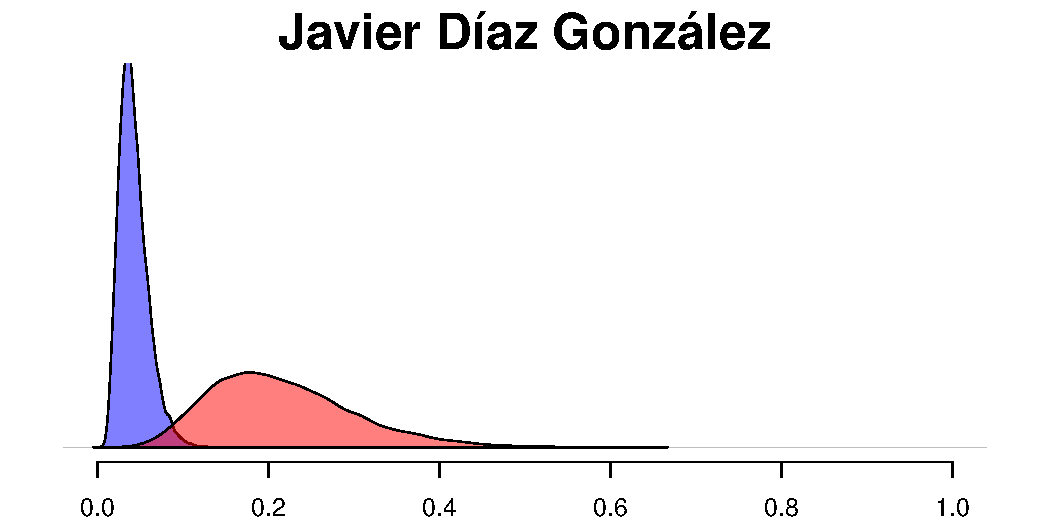
\includegraphics[width=.3\columnwidth]{../graphs/prReconoce1.pdf} &
%     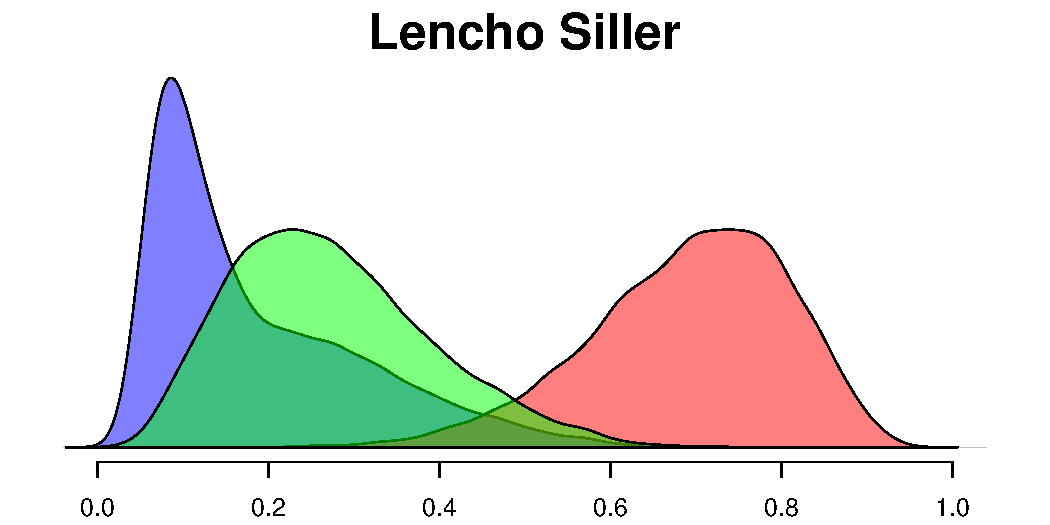
\includegraphics[width=.3\columnwidth]{../graphs/prReconoce6.pdf} &
%     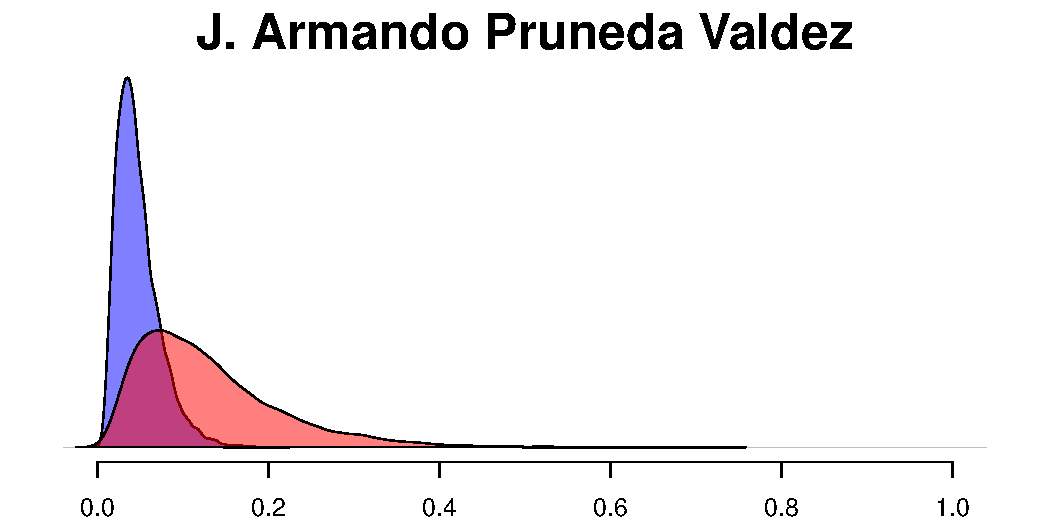
\includegraphics[width=.3\columnwidth]{../graphs/prReconoce8.pdf} \\
%     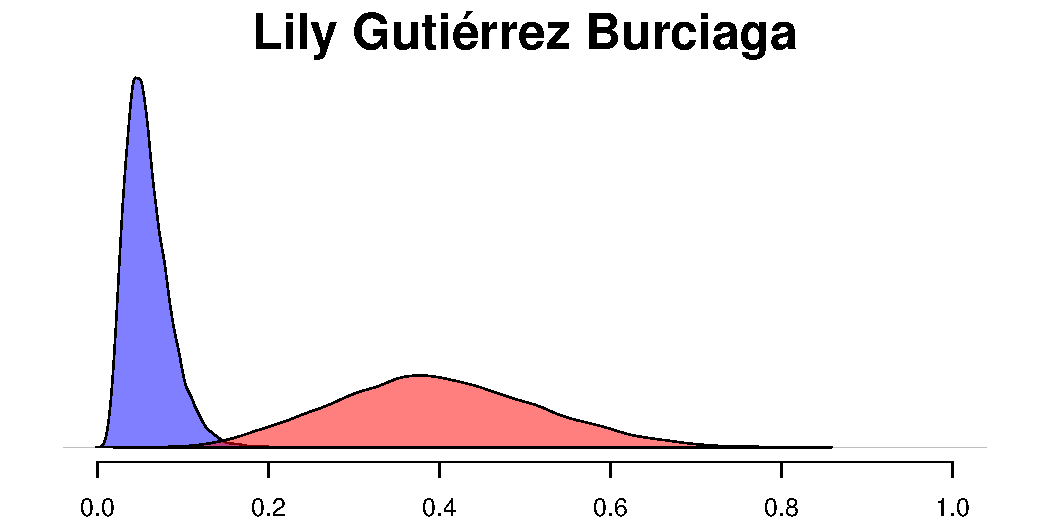
\includegraphics[width=.3\columnwidth]{../graphs/prReconoce2.pdf} &
%     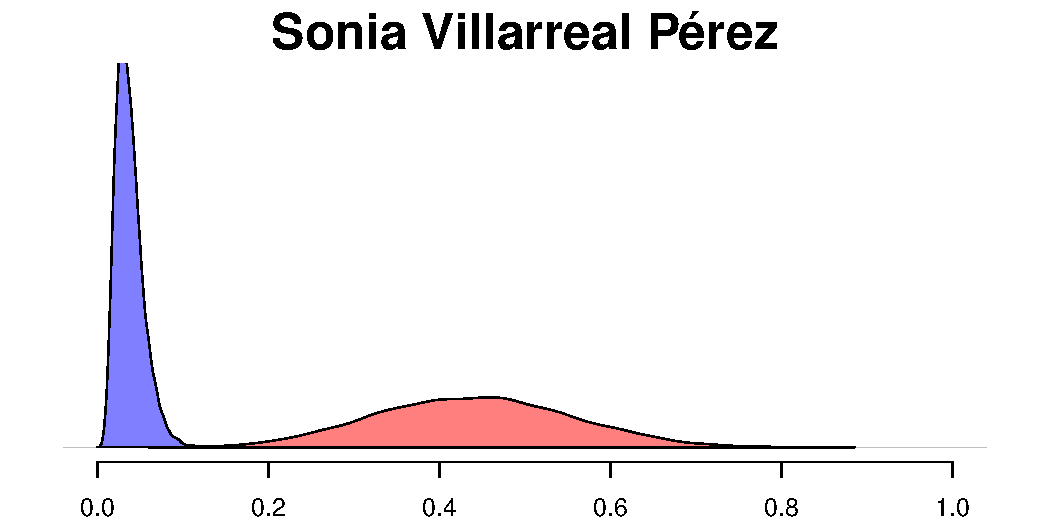
\includegraphics[width=.3\columnwidth]{../graphs/prReconoce5.pdf} &
%     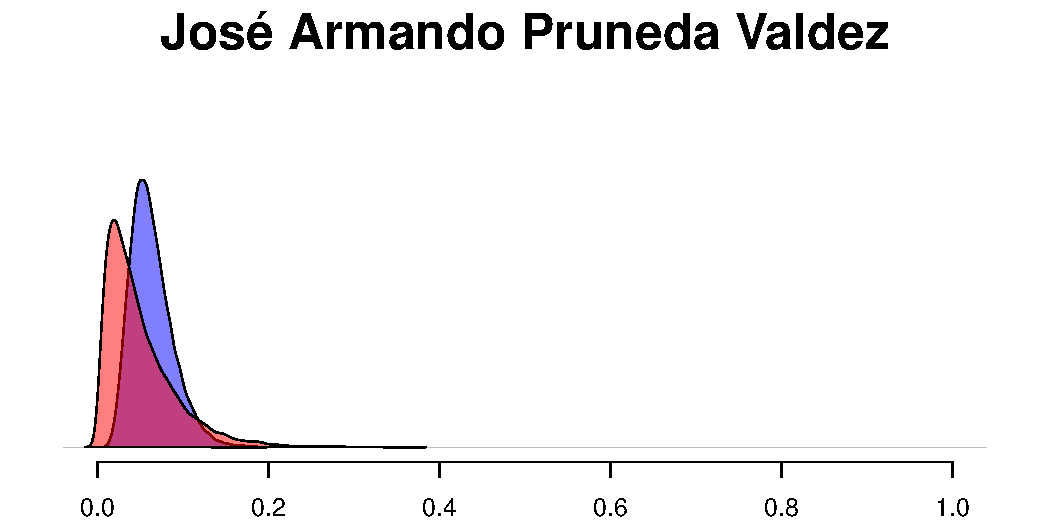
\includegraphics[width=.3\columnwidth]{../graphs/prReconoce7.pdf} \\
%     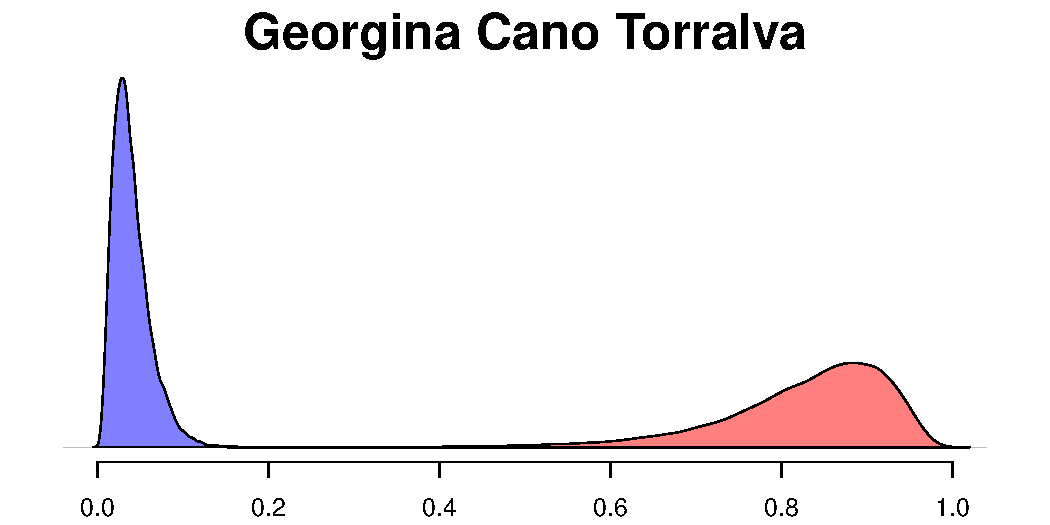
\includegraphics[width=.3\columnwidth]{../graphs/prReconoce3.pdf} &
%     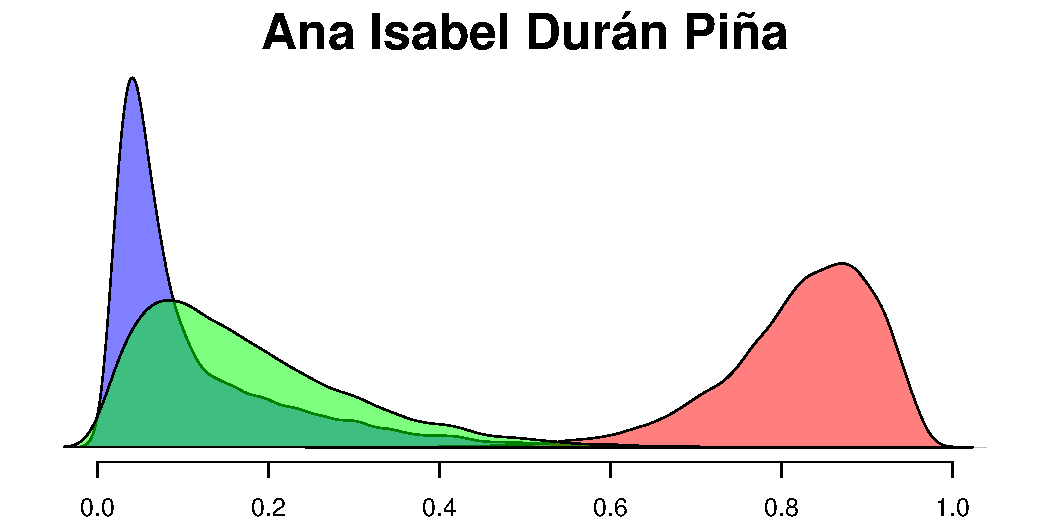
\includegraphics[width=.3\columnwidth]{../graphs/prReconoce4.pdf} &
%     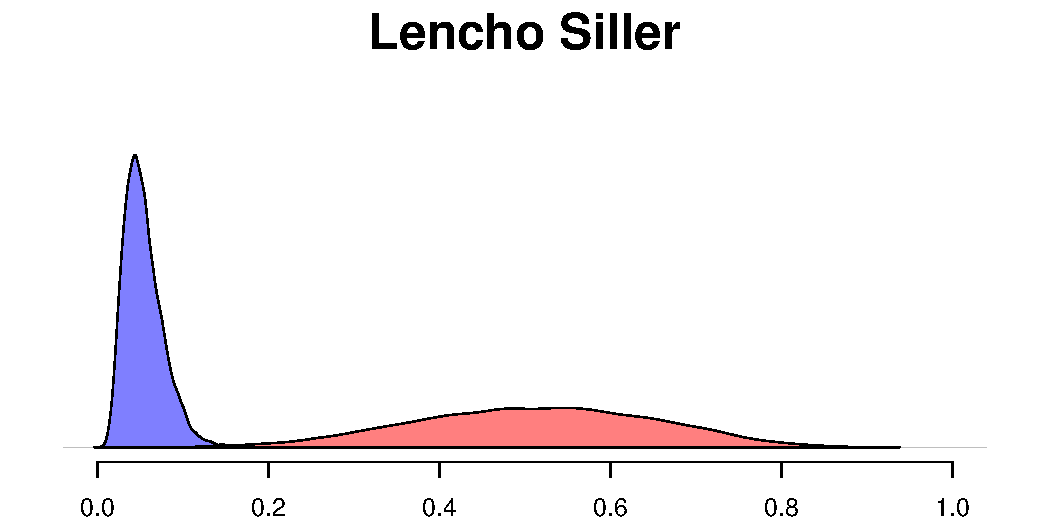
\includegraphics[width=.3\columnwidth]{../graphs/prReconoce9.pdf} \\
%   \end{tabular}
% ~ \\
% ~ \\
% %\definecolor{MidnightBlue}{rgb}{0.1, 0.1, 0.44}
% \definecolor{MidnightBlue}{rgb}{0.48, 0.41, 0.93}
% \definecolor{LimeGreen}{rgb}{0.2, 0.8, 0.2}
% \definecolor{Salmon}{rgb}{1.0, 0.55, 0.41}
% \begin{large}
% \textbf{Hypotheses}:
% \begin{tabular}{|rc|}
% \hline  incumbency & \textcolor{MidnightBlue}{$n$} $<$ \textcolor{LimeGreen}{$l$} $<$ \textcolor{Salmon}{$r$} \\
%   campaign   & \textcolor{MidnightBlue}{$n$} $=$ \textcolor{LimeGreen}{$l$} $<$ \textcolor{Salmon}{$r$} \\ \hline
% \end{tabular}
% \end{large}
% \caption{The probability of name recognition (x-axis). We portray simulations with Bayesian versions of regression models. The violet density is for respondents in area $n$, the green (when applicable) for respondents in area $l$, and the pink for respondents in area $r$. \emph{With clear gaps between them, we expect the purple to lie to the left, the pink to the right, the green between them}. All other controls held constant to represent a PAN-identifier with a smartphone, who said the incumbent has delivered but is uninterested in politics.}\label{f:sims}
% \end{sidewaysfigure}

\begin{figure}
  \centering
  \begin{tabular}{cc}
    Static ambition & Progressive ambition \\ \hline
    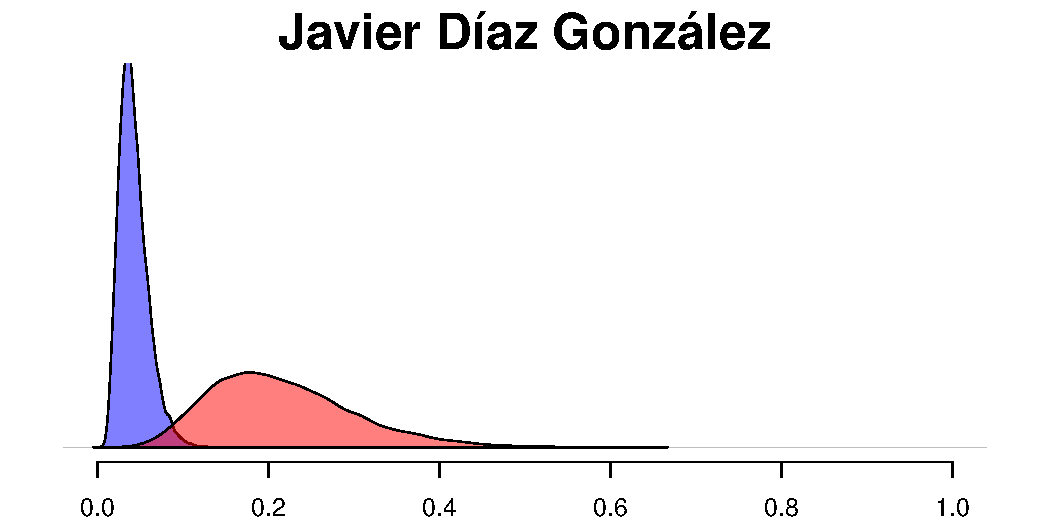
\includegraphics[width=.3\columnwidth]{../graphs/prReconoce1.pdf} &
    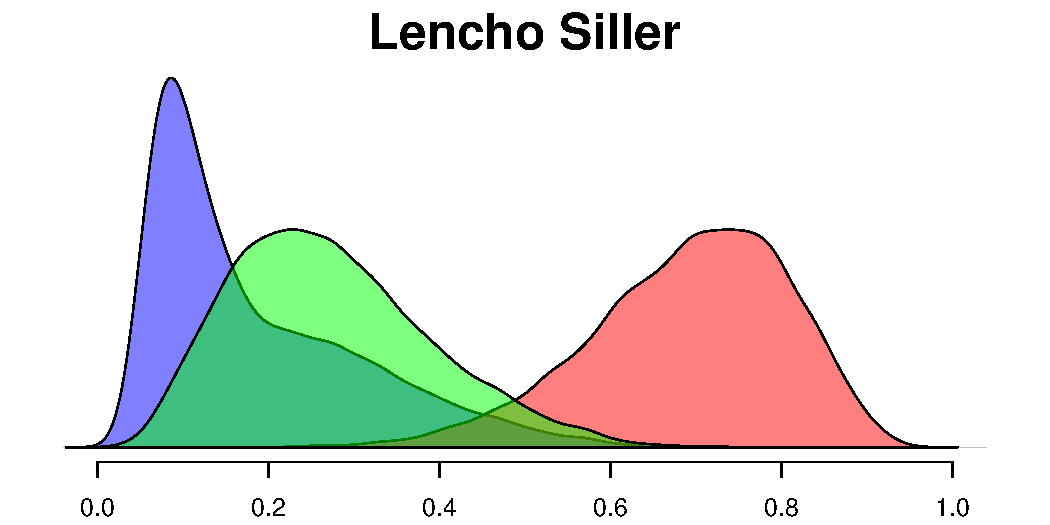
\includegraphics[width=.3\columnwidth]{../graphs/prReconoce6.pdf} \\
    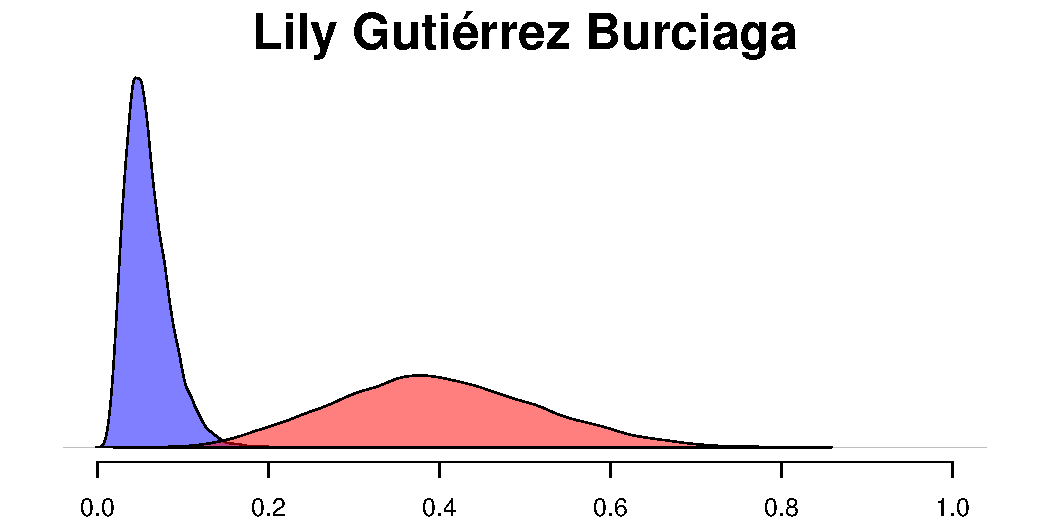
\includegraphics[width=.3\columnwidth]{../graphs/prReconoce2.pdf} &
    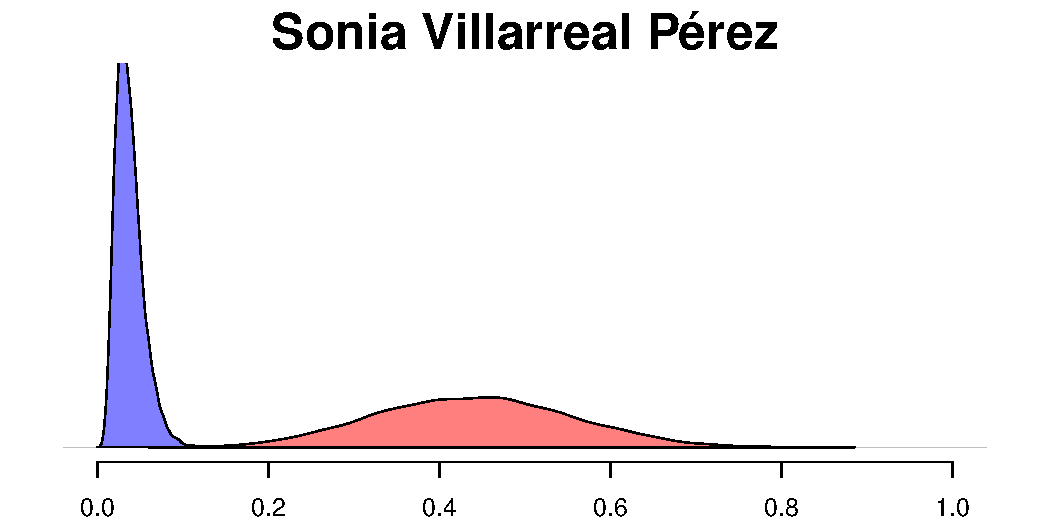
\includegraphics[width=.3\columnwidth]{../graphs/prReconoce5.pdf} \\
    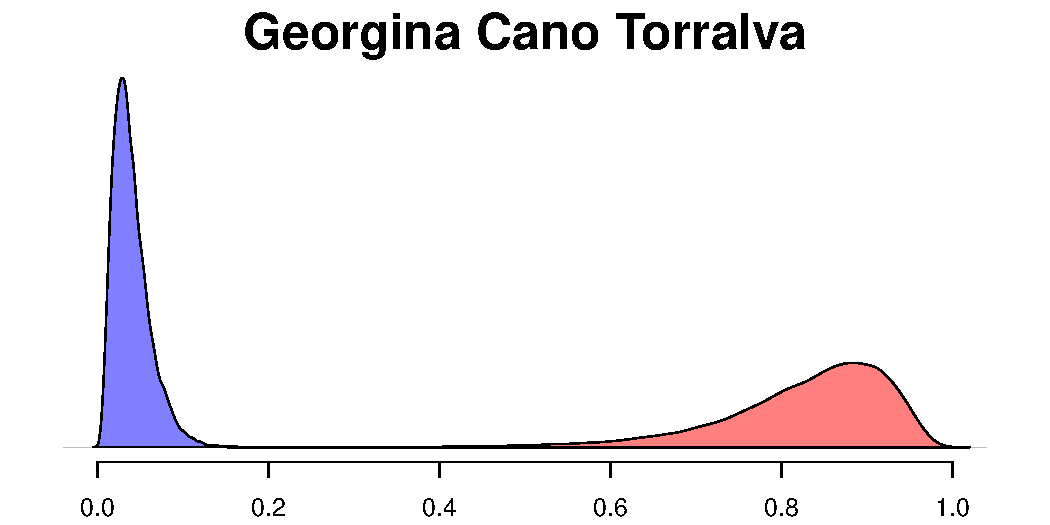
\includegraphics[width=.3\columnwidth]{../graphs/prReconoce3.pdf} &
    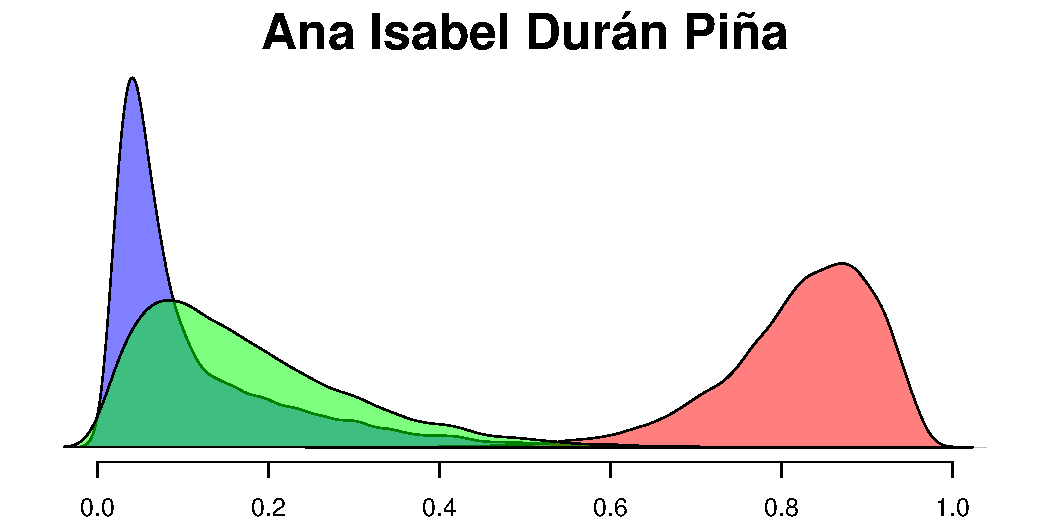
\includegraphics[width=.3\columnwidth]{../graphs/prReconoce4.pdf} \\
  \end{tabular}
~ \\ ~ \\ ~ \\
%\definecolor{MidnightBlue}{rgb}{0.1, 0.1, 0.44}
\definecolor{MidnightBlue}{rgb}{0.48, 0.41, 0.93}
\definecolor{LimeGreen}{rgb}{0.2, 0.8, 0.2}
\definecolor{Salmon}{rgb}{1.0, 0.55, 0.41}
\begin{tabular}{|rc|}
  \hline \multicolumn{2}{|c|}{\textbf{Hypotheses}:} \\
  incumbency & \textcolor{MidnightBlue}{$n$} $<$ \textcolor{LimeGreen}{$l$} $=$ \textcolor{Salmon}{$r$} \\
  campaign   & \textcolor{MidnightBlue}{$n$} $=$ \textcolor{LimeGreen}{$l$} $<$ \textcolor{Salmon}{$r$} \\ \hline
\end{tabular}
\caption{The probability of name recognition (x-axis). Simulations generated with Bayesian estimations of regression models. The violet density is for respondents in area $n$, the green (when applicable) for respondents in area $l$, and the pink for respondents in area $r$. Incumbency leads to expect the purple to lie to the left, the pink to the right, the green between them, with clear gaps between them. All other controls held constant to represent a PAN-identifier with a smartphone, who said the incumbent has delivered but is uninterested in politics.}\label{f:sims}
\end{figure}

Simulations reveal effects neatly in Figure \ref{f:sims}. The curves are posterior probabilities of name recognition from a Bayesian re-estimation of the logit models. Colored densities hold predictors constant except redistricting areas dummies. A gap is expected, and observed across the board, between the violet and pink densities, corresponding respectively to voters in low-probability area $n$ and higher-probability area $r$. Incumbency hypotheses expect the green density, for voters in area $l$, to overlap with the right-side density, campaign hypotheses with the left-side density. Plots show how separation is not as clear cut as statistically significant results might otherwise suggest. There is substantive overlap of green and pink in Javier Díaz González's case, but the green--violet overlap is important too. Plots also reveal that, among the progressively ambitious, green overlaps much more with violet than pink. Throughout their terms, State Deputies Lencho Siller and Ana Isabel Durán Piña seem to have devoted a good deal of effort servicing the municipalities they ran in---the ``retained'' parts---hence the name recognition hike relative to district ``lost''.

\section{Conclusion}

Our investigation of name familiarity in Coahuila has achieved a number of things. We discussed how the electoral connection, by inducing politicians with static ambition to cultivate a personal vote by trading in particularistic goods, should heighten levels of name recognition among constituents. We also saw admonitions (skeptics' warning) of minimal effects in Mexico, as reformers chose to keep parties' firm grip on nominations in place and politicans in Latin America have proverbial lack of static ambition. So are there signs of an electoral connection in Coahuila's 2017 state legislative races, where incumbents were allowed to seek consecutive reelection for the first time in over eight decades? On top of admonitions (warnings), differentials in name familiarity could be due to campaigns, not the personal vote. 

The paper develops a method to overcome this obstacle by exploiting redistricting. Changes in the electoral geography are means to separate incumbency from campaign effects in name recognition. We set forth resolving these issues empirically with an original pre-election survey in the state. If unable to totally rule out the effect of campaigns, the public opinion evidence we produce does reveal statistically significant and substantive total effects in name recognition consistent with the personal vote. This is a noteworthy and important finding. 

- It paves the way for an in-depth study of reelection in Mexico. If Coahuila revealed interesting patterns despite limitations, the agenda ahead is promising. N congressional candidates in 2018 and 2021. N municipal.  

- If small in scope, our study constitutes a rare attempt to measure the mass component of the personal vote outside the U.S. and the U.K. 
Need cross-sectional and cross-temporal approaches in future research. 

- The separation method applicable to other cases where district boundaries are routinely adjusted to counter malapportionment.  

\bibliographystyle{apsrInitials}
\bibliography{/home/eric/Dropbox/mydocs/magar}

\newpage
\section{Appendix}

\subsection{Descriptive statistics: survey}

Unlike absolute frequencies In the summaries below, relative frequencies are parenthesized (reporting percentages). All missing answers are reported (NS/NC = ``No Answer/Don't Know''), so totals add to 1,008 respondents for all survey questions. Percentages may not add to 100 exactly due to rounding. The summary for `Localidad' illustrates, afterwards labels are omitted for economy. Section \ref{s:tran} includes an English translation of the survey questions about consecutive reelection. 

\begin{scriptsize}
\begin{verbatim}
Localidad
   Urbana         Rural         Mixta        Total
  N    (%)      N    (%)      N    (%)      N    (%)
----------------------------------------------------
840   (83)     70    (7)     98   (10)   1008  (100)

Municipio (% only)
            ABASOLO               ACUÑA             ALLENDE             ARTEAGA 
             (0.00)              (5.56)              (0.00)              (0.00) 
            CANDELA            CASTAÑOS      CUATROCIENEGAS            ESCOBEDO 
             (0.00)              (1.39)              (1.39)              (0.00) 
FRANCISCO I. MADERO            FRONTERA      GENERAL CEPEDA            GUERRERO 
             (1.39)              (2.78)              (1.39)              (0.00) 
            HIDALGO             JIMENEZ              JUAREZ            LAMADRID 
             (0.00)              (1.39)              (0.00)              (0.00) 
          MATAMOROS            MONCLOVA             MORELOS             MUZQUIZ 
             (4.17)              (6.94)              (0.00)              (2.78) 
          NADADORES                NAVA              OCAMPO              PARRAS 
             (0.00)              (1.39)              (0.00)              (1.39) 
     PIEDRAS NEGRAS            PROGRESO        RAMOS ARIZPE             SABINAS 
             (5.56)              (0.00)              (2.78)              (2.78) 
         SACRAMENTO            SALTILLO    SAN BUENAVENTURA SAN JUAN DE SABINAS 
             (0.00)             (26.39)              (1.39)              (1.39) 
          SAN PEDRO       SIERRA MOJADA             TORREON              VIESCA 
             (4.17)              (0.00)             (23.61)              (0.00) 
        VILLA UNION            ZARAGOZA               Total
             (0.00)              (0.00)            (100.00)

Sección electoral (N only)
   4    8   10   84  119  141  192  197  214  242  258  263  269  325  328  370 
-------------------------------------------------------------------------------
  14   14   14   14   14   14   14   14   14   14   14   14   14   14   14   14 
===============================================================================
 378  411  454  473  508  550  580  586  617  627  653  661  692  712  734  737 
-------------------------------------------------------------------------------
  14   14   14   14   14   14   14   14   14   14   14   14   14   14   14   14 
===============================================================================
 788  800  816  843  847  869  871  897  905  907  920  922  932  977  979 1042 
-------------------------------------------------------------------------------
  14   14   14   14   14   14   14   14   14   14   14   14   14   14   14   14 
===============================================================================
1068 1109 1145 1157 1173 1184 1214 1221 1263 1272 1303 1314 1316 1351 1377 1388 
-------------------------------------------------------------------------------
  14   14   14   14   14   14   14   14   14   14   14   14   14   14   14   14 
===============================================================================
1402 1447 1449 1464 1469 1623 1678 1703  Total
-------------------------------------------------------------------------------
  14   14   14   14   14   14   14   14   1008

Congressional district
       1        2        3        4        5        6        7      Total
-------------------------------------------------------------------------
140 (14) 154 (15) 154 (15) 154 (15) 140 (14) 154 (15) 112 (11) 1008 (100) 

State assembly district
     1      2      3      4      5      6      7      8      9     10     11     12     13  
------------------------------------------------------------------------------------------
70 (7) 70 (7) 70 (7) 70 (7) 56 (6) 56 (6) 56 (6) 70 (7) 84 (8) 42 (4) 42 (4) 56 (6) 84 (8) 
==========================================================================================
     14     15     16      Total
--------------------------------
 56 (6) 84 (8) 42 (4) 1008 (100)

(Si tiene credencial para votar vigente) ¿Está registrada en este domicilio o en otro?
   En este        En otro
-------------------------
813   (81)     195   (19) 

Sexo
   Hombre        Mujer
----------------------
502  (50)    506  (50)
 
Edad (grouped)
 [18,28)   [28,38)   [38,48)   [48,58)   [58,68)    [68,+)
----------------------------------------------------------         
211 (21)  205 (20)  203 (20)  180 (18)  117 (12)   92  (9)

 
1 En su opinión, ¿cuál es el principal problema que hay actualmente en el Estado de 
Coahuila? (ANOTAR TEXTUAL)                   (%)
------------------------------------------------
                                  Campo    (0.2) 
                             Corrupción   (13.7) 
                              Desempleo   (12.4) 
                               Economía    (6.5) 
                              Educación    (0.8) 
            Falta de buenos gobernantes    (0.9) 
                    Fenómenos naturales    (0.1) 
Inflación/alza de precios/precios altos    (0.8) 
                    Inseguridad pública   (45.0) 
                           Narcotráfico    (1.0) 
                                Ninguno    (1.0) 
                         Obras públicas    (0.4) 
                                Pobreza    (3.1) 
                    Problemas políticos    (0.5) 
                        Gobierno de epn    (0.3) 
                     Problemas sociales    (1.1) 
                                  Salud    (0.9) 
                     Servicios públicos    (9.7) 
                                  Todos    (1.0) 
                                  Otros    (0.4) 
              Falta de ayuda a la gente    (0.2) 
          Demasiados programas sociales    (0.1) 

2 Por lo general, ¿cuánto le interesa la política? (LEER)
     Mucho         Algo         Poco         Nada        NS/NC
--------------------------------------------------------------
122 (12.1)   259 (25.7)   324 (32.1)   301 (29.9)     2  (0.2) 

3 ¿Sabe cuándo son las próximas elecciones para Gobernador del estado? 
(NO LEER: 4 DE JUNIO 2017)
Sabe completa    Incompleta        NS/NC 
----------------------------------------
    719  (71)    160   (16)    129  (13) 

4 Del 0 a 10, donde 0 es nada probable y 10 muy probable, ¿qué tan probable es que 
usted vote en las próximas elecciones para gobernador?
        0         1         2         3         4         5 
---------------------------------------------------------------
 64 (6.3)  37 (3.7)  21 (2.1)  25 (2.5)  14 (1.4)  90 (8.9)
===============================================================
        6         7          8         9          10      NS/NC
----------------------------------------------------------------
 36 (3.6)  50 (5.0) 113 (11.2)  49 (4.9)  505 (50.1)     4 (0.4) 
         
5 (USAR BOLETA 1) Si hoy hubiera elecciones para Gobernador del estado, ¿por 
quién votaría                            N       (%)
----------------------------------------------------
               Guillermo Anaya, PAN    194    (19.2) 
             Miguel A. Riquelme,PRI    238    (23.6) 
              Mary T. Guajardo, PRD     15     (1.5) 
                  José A. Pérez, PT     15     (1.5) 
           Miguel A. Riquelme, PVEM     16     (1.6) 
               Guillermo Anaya, UDC     14     (1.4) 
          Miguel A. Riquelme, PANAL      8     (0.8) 
            Miguel A. Riquelme, PSI      4     (0.4) 
               Guillermo Anaya, PPC      2     (0.2) 
  Miguel A. Riquelme, Partido Jóven      9     (0.9) 
            Miguel A. Riquelme, PRC      3     (0.3) 
            Miguel A. Riquelme, PCP      4     (0.4) 
           Armando Guadiana, Morena    102    (10.1) 
  Guillermo Anaya, Encuentro Social      7     (0.7) 
     Javier Guerrero, Independiente     45     (4.5) 
Luis Horacio Salinas, Independiente     12     (1.2) 
                      No registrado      5     (0.5) 
                               Nulo     88     (8.7) 
                            Ninguno     52     (5.2) 
                              NS/NC    175    (17.4) 
                              TOTAL   1008   (100.0)

6 ¿Usted ya decidió definitivamente por quién votar para gobernador, 
tiene idea pero podría cambiar o aún no decide su voto?
                                N     (%)
-----------------------------------------
Ya decidió definitivamente    558    (55)
Tiene idea, podría cambiar    150    (15)
             Aún no decide    246    (24)
                     NS/NC     54     (5) 

7 ¿Cuál es su opinión acerca de los siguientes personajes políticos: muy buena, buena, mala, 
muy mala,... o no lo conoce suficiente para opinar? (LEER Y ROTAR NOMBRES)

a Guillermo Anaya Llamas       
    Muy                             Muy    Ni buena               No lo  
  buena     Buena       Mala       mala     ni mala      NS/NC   conoce       Total
-----------------------------------------------------------------------------------
 41 (4)  260 (26)   191 (19)   106 (11)    260 (26)   100 (10)   50 (5)  1008 (100)  
 
b Miguel Ángel Riquelme        
    Muy                             Muy    Ni buena               No lo  
  buena     Buena       Mala       mala     ni mala     NS/NC    conoce      Total
----------------------------------------------------------------------------------
 45 (4)  224 (22)   225 (22)   187 (19)    195 (19)    93 (9)    39 (4)  1008 (100) 

c Mary Telma Guajardo Villareal
    Muy                             Muy    Ni buena               No lo  
  buena     Buena       Mala       mala     ni mala     NS/NC    conoce      Total
----------------------------------------------------------------------------------
  3 (0)    77 (8)    96 (10)     64 (6)    162 (16)   254 (25) 352 (35)  1008 (100)

d José Ángel Pérez Hernández   
    Muy                             Muy    Ni buena               No lo  
  buena     Buena       Mala       mala     ni mala     NS/NC    conoce      Total
----------------------------------------------------------------------------------
 15 (1)    95 (9)     95 (9)     76 (8)    164 (16)   274 (27) 289 (29)  1008 (100)

e Armando Guadiana Tijerina    
    Muy                             Muy    Ni buena               No lo  
  buena     Buena       Mala       mala     ni mala     NS/NC    conoce      Total
----------------------------------------------------------------------------------
 21 (2)  159 (16)   88   (9)   71   (7)   180  (18)  210 (21)  279 (28)  1008 (100)

f Javier Guerrero García       
    Muy                             Muy    Ni buena               No lo  
  buena     Buena       Mala       mala     ni mala     NS/NC    conoce      Total
----------------------------------------------------------------------------------
 16 (2)  137 (14)     74 (7)     61 (6)    180 (18)  256 (25)  284 (28)  1008 (100)

g Luis Horacio Salinas Valdez  
    Muy                             Muy    Ni buena               No lo  
  buena     Buena       Mala       mala     ni mala     NS/NC    conoce      Total
----------------------------------------------------------------------------------
  6 (1)    56 (6)     71 (7)     60 (6)    138 (14)   284 (28) 393 (39)  1008 (100) 

8 ¿Si la elección para gobernador solamente fuera entre Guillermo Anaya y Miguel 
Riquelme, ¿por quién votaría usted?                          N   (%)
--------------------------------------------------------------------
                    Guillermo Anaya del PAN-UDC-PPC-PES   334   (33) 
Miguel Ángel Riquelme del PRI-PVEM-PANAL-PSI-PJ-PRC-PCP   314   (31) 
                                                Ninguno   273   (27) 
                                                  NC/NC    87    (9) 

9 ¿Quién cree que gane la elección para gobernador? (LEER)
Guillermo Anaya del PAN  Miguel Ángel Riquelme del PRI    Otro       NS/NC
--------------------------------------------------------------------------
               258 (26)                       487 (48)    0 (0)   263 (26) 

10 De los siguientes asuntos que le voy a leer, dígame por favor cuál es el 
más importante que debe atender el próximo gobernador del estado: 
(LEER)                   N   (%)
--------------------------------
        Inseguridad    319  (32)
            Pobreza    193  (19)
            Empleos    170  (17)
         Corrupción    170  (17)
          Educación     41   (4)
     Medio ambiente     10   (1)
La deuda del estado     66   (7)
               Otro      0   (0)
              NS/NC     39   (4)
 
11 (USAR BOLETA 2) Si hoy hubiera elecciones para Diputados Locales, ¿por cuál partido 
votaría usted?
     PAN      PRI     PRD      PT    PVEM     UDC     MC   PANAL    PSI    PPC 
------------------------------------------------------------------------------
206 (20) 264 (26)  16 (2)  20 (2)  17 (2)  23 (2)  6 (1)  13 (1)  1 (0)  7 (1) 
==============================================================================
     PJ     PRC     PCP  MORENA    PES  Independiente       <NA>       Total
----------------------------------------------------------------------------
 15 (1)   3 (0)   6 (1)  88 (9)  5 (0)         35 (3)   283 (28)  1008 (100)

12 (USAR BOLETA 3) Si hoy hubiera elecciones para Presidente Municipal, ¿por cuál partido 
votaría usted?
     PAN      PRI     PRD      PT    PVEM     UDC     MC   PANAL    PSI    PPC 
------------------------------------------------------------------------------
218 (22) 287 (28)  17 (2)  14 (1)  11 (1)  22 (2)  8 (1)   5 (0)  1 (0)  9 (1) 
==============================================================================
     PJ     PRC     PCP  MORENA    PES  Independiente       <NA>       Total
----------------------------------------------------------------------------
 13 (1)   2 (0)   6 (1)  78 (8)  5 (0)          38 (4)  274 (27)  1008 (100)

13 ¿Votó usted en las elecciones para gobernador en julio de 2011? (SÍ) 
¿Por quién votó usted? (LEER OPCIONES)     N     (%)
----------------------------------------------------
      Guillermo Anaya Llamas, PAN-UDC    211    (21) 
Rubén Moreira, PRI-PVEM-PANAL-PPC-PSI    367    (36) 
                                 Otro      0     (0) 
                        No registrado     22     (2) 
                                 Nulo     21     (2) 
                              No votó    255    (25) 
                                NS/NC    132    (13) 

14 En general, ¿usted aprueba o desaprueba el trabajo que Rubén Moreira está haciendo 
como Gobernador del estado? (INSISTIR): ¿APRUEBA/DESAPRUEBA mucho o algo?
Aprueba mucho    Aprueba algo   Desaprueba algo   Desaprueba mucho    NS/NC 
---------------------------------------------------------------------------
       88 (9)        294 (29)          233 (23)           357 (35)   36 (4) 

15 En general, ¿está satisfecho o insatisfecho con la manera en que marchan las cosas 
en el estado? (INSISTIR: ¿Muy o algo?) (5=NS/NC)
Muy satisfecho    Algo satisfecho    Algo satisfecho    Muy insatisfecho     NS/NC
----------------------------------------------------------------------------------
        52 (5)           329 (33)           318 (32)            297 (29)    12 (1) 

16 En general, ¿usted aprueba o desaprueba el trabajo que Enrique Peña Nieto está 
haciendo como Presidente de la República? (INSISTIR): ¿APRUEBA/DESAPRUEBA mucho o algo?
Aprueba mucho    Aprueba algo   Desaprueba algo   Desaprueba mucho    NS/NC 
---------------------------------------------------------------------------
       72 (7)        199 (20)          184 (18)           531 (53)   22 (2) 

17 ¿Cómo calificaría en estos momentos... (LEER):? muy bien, bien, mal o muy mal?

a La situación económica del estado
Muy bien      Bien       Mal    Muy mal   Ni bien ni mal    NS/NC 
-----------------------------------------------------------------
  10 (1)  164 (16)  319 (32)   330 (33)         182 (18)    3 (0) 

b Su situación económica familiar
Muy bien      Bien       Mal    Muy mal   Ni bien ni mal    NS/NC 
-----------------------------------------------------------------
  20 (2)  344 (34)  231 (23)   130 (13)         282 (28)    1 (0) 

c La seguridad pública en la comunidad donde vive
Muy bien      Bien       Mal    Muy mal   Ni bien ni mal    NS/NC 
-----------------------------------------------------------------
  33 (3)  290 (29)  277 (27)   223 (22)         177 (18)    8 (1) 

18 Generalmente, ¿usted se considera priista, panista, perredista morenista? (INSISTIR): 
¿Se considera muy o algo?
       Priista        Panista       Perredista     Morenista
     muy     algo    muy   algo    muy    algo     muy    algo   NS/NC    Otro  Ninguno
---------------------------------------------------------------------------------------
151 (15) 101 (10) 70 (7) 43 (4)  9 (1)   3 (0)  23 (2)  22 (2)   0 (0) 538 (53)  48 (5) 

19 (TARJETA 1) En política la gente habla de “la izquierda” y “la derecha”. En general, 
¿cómo colocaría usted sus puntos de vista en esta escala, donde 1 es izquierda y 10 es 
derecha? También puede escoger un punto intermedio.
       1      2      3      4        5      6      7      8      9       10    NS/NC 
------------------------------------------------------------------------------------
115 (11) 29 (3) 52 (5) 48 (5) 214 (21) 87 (9) 49 (5) 79 (8) 32 (3) 127 (13) 176 (17) 

20 ¿Está usted a favor, en contra o le es indiferente la reelección consecutiva de 
legisladores?
 A favor  En contra  Le es indiferente   NS/NC 
----------------------------------------------
121 (12)   511 (51)           320 (32)  56 (6) 

21 El 3 de abril iniciaron las campañas para renovar el Congreso del Estado. Si yo le 
preguntara los nombres de los candidatos a diputado en este distrito, ¿usted me podría 
decir todos los nombres, algunos nombres o no recuerda ningún nombre en este momento?
Todos   Algunos  No recuerda  No contestó 
-----------------------------------------
9 (1)  144 (14)     783 (78)       72 (7) 

22 Ahora piense por favor en los diputados locales actuales. Si yo le preguntara las 
cosas que ha hecho su diputado por esta comunidad, ¿usted podría mencionarme muchas cosas, 
algunas, diría que no hizo nada o no recuerda en este momento?
Muchas   Algunas   No hizo nada   No recuerda    NS/NC
------------------------------------------------------
18 (2)  217 (22)       495 (49)      266 (26)   12 (1) 

23 Si su actual diputado compitiera para buscar la reelección, ¿usted votaría por él 
o no votaría por él?
Sí votaría por él   No votaría por él      NS/NC 
------------------------------------------------
         156 (15)            731 (73)   121 (12) 

24 Con base en el trabajo realizado por su actual diputado, ¿cree que merecería ser 
reelecto en su cargo o no?
      Sí        No        NC 
----------------------------
158 (16)  751 (75)   99 (10) 

25 Le voy a leer unos nombres, para cada uno, ¿podría decirme si le es muy conocido, 
algo conocido, poco o nada conocido?

a Javier Díaz González     
Muy conocido     Algo     Poco   Nada conocido    NS/NC 
-------------------------------------------------------
      17 (2)   30 (3)   36 (4)        889 (88)   36 (4) 

b Lily Gutiérrez Burciaga  
Muy conocido     Algo     Poco   Nada conocido    NS/NC 
-------------------------------------------------------
      14 (1)   34 (3)   29 (3)        895 (89)   36 (4) 

c Georgina Cano Torralva   
Muy conocido     Algo     Poco   Nada conocido    NS/NC 
-------------------------------------------------------
      22 (2)   40 (4)   24 (2)        884 (88)   38 (4) 

d Ana Isabel Durán         
Muy conocido     Algo     Poco   Nada conocido    NS/NC 
-------------------------------------------------------
      10 (1)   34 (3)   25 (2)        901 (89)   38 (4) 

e Sonia Villareal          
Muy conocido     Algo     Poco   Nada conocido    NS/NC 
-------------------------------------------------------
      20 (2)   41 (4)   22 (2)        888 (88)   37 (4) 

f Lariza Montiel           
Muy conocido     Algo     Poco   Nada conocido    NS/NC 
-------------------------------------------------------
      18 (2)   33 (3)   13 (1)        906 (90)   38 (4) 

g Armando Pruneda          
Muy conocido     Algo     Poco   Nada conocido    NS/NC 
-------------------------------------------------------
       6 (1)   20 (2)   10 (1)        933 (93)   39 (4) 

h Leonel Contreras Pámanes 
Muy conocido     Algo     Poco   Nada conocido    NS/NC 
-------------------------------------------------------
       6 (1)   25 (2)   25 (2)        912 (90)   40 (4) 

i Florencio "Lencho" Siller
Muy conocido     Algo     Poco   Nada conocido    NS/NC 
-------------------------------------------------------
       7 (1)   29 (3)   31 (3)        902 (89)   39 (4) 

26 En los últimos 12 meses, ¿usted o alguien de su familia... (LEER)

a Perdió su empleo o fuente de ingresos económicos?
Sí, usted   Sí, un familiar   Sí, ambos        No     NS/NC 
-----------------------------------------------------------
 141 (14)          212 (21)      17 (2)  635 (63)     3 (0) 

b Fue víctima de algún delito o un asalto?
Sí, usted   Sí, un familiar   Sí, ambos        No     NS/NC 
-----------------------------------------------------------
  97 (10)            93 (9)      20 (2)  796 (79)     2 (0) 

c Tuvo que dar alguna mordida
Sí, usted   Sí, un familiar   Sí, ambos        No     NS/NC 
-----------------------------------------------------------
  99 (10)            54 (5)      12 (1)  839 (83)     4 (0) 

27 Por lo general, ¿cuánto se entera de las noticias por medio de... (LEER), 
mucho, algo, poco o nada?

a Televisión
   Mucho       Algo       Poco       Nada      NS/NC 
----------------------------------------------------
413 (41)   242 (24)   228 (23)   123 (12)      2 (0) 

b Radio
   Mucho       Algo       Poco       Nada      NS/NC 
----------------------------------------------------
188 (19)   222 (22)   190 (19)   404 (40)      4 (0) 

c Periódico
   Mucho       Algo       Poco       Nada      NS/NC 
----------------------------------------------------
132 (13)   167 (17)   173 (17)   530 (53)      6 (1) 

d Pláticas con gente
   Mucho       Algo       Poco       Nada      NS/NC 
----------------------------------------------------
190 (19)   271 (27)   183 (18)   355 (35)      9 (1) 

e Internet
   Mucho       Algo       Poco       Nada      NS/NC 
----------------------------------------------------
274 (27)   149 (15)    99 (10)   474 (47)     12 (1) 

f Redes sociales
   Mucho       Algo       Poco       Nada      NS/NC 
----------------------------------------------------
278 (28)   153 (15)    82  (8)   482 (48)     13 (1) 

28 ¿Utiliza Facebook?
      Sí       No      NC
-------------------------
559 (55) 444 (44)   5 (0) 

29 ¿Utiliza Twitter?
      Sí       No      NC
-------------------------
138 (14) 868 (86)   2 (0) 

30 ¿Tiene Smartphone o teléfono inteligente?
      Sí       No      NC
-------------------------
562 (56) 441 (44)   5 (0) 

31 ¿Usted o alguien en su hogar es beneficiario de... (LEER)?

a Oportunidades/Prospera
Sí, usted    Sí, un familiar     Sí, ambos           No       NS/NC
-------------------------------------------------------------------
   94 (9)            98 (10)        10 (1)     797 (79)       9 (1) 

b Seguro Popular
Sí, usted    Sí, un familiar     Sí, ambos           No       NS/NC
-------------------------------------------------------------------
 162 (16)             84 (8)        67 (7)     688 (68)       7 (1) 

c Algún programa social del gobierno del estado
Sí, usted    Sí, un familiar     Sí, ambos           No       NS/NC
-------------------------------------------------------------------
 120 (12)             65 (6)        11 (1)     802 (80)      10 (1) 

32 Durante estas campañas electorales, ¿a usted o alguien en su hogar... (LEER)?

a Le han dado algún obsequio los partidos o candidatos
Sí, usted    Sí, un familiar     Sí, ambos           No       NS/NC
-------------------------------------------------------------------
 110 (11)             67 (7)        25 (2)     803 (80)       3 (0) 

b Ha asistido a eventos de los partidos o candidatos
Sí, usted    Sí, un familiar     Sí, ambos           No       NS/NC
-------------------------------------------------------------------
 135 (13)             52 (5)       22  (2)     796 (79)       3 (0) 

33 Si los candidatos a la Presidencia de la República en 2018 fueran los siguientes, 
¿por quién votaría usted? (LEER Y ROTAR)

[[NOT INCLUDED IN DATABASE???]]

34 ¿Cuál es su opinión acerca de los siguientes personajes políticos: muy buena, 
buena, mala, muy mala,... o no lo conoce suficiente para opinar? (LEER Y ROTAR NOMBRES)
a Andrés Manuel López Obrador
b Margarita Zavala
c Miguel Ángel Osorio Chong
d Humberto Moreira

[[NOT INCLUDED IN DATABASE???]]

35 Juntando el dinero que usted y otros miembros de su familia ganan al mes, 
¿diría que...? (LEER)
                            Les alcanza bien    207    (21) 
        Les alcanza con algunas dificultades    459    (46) 
                              No les alcanza    238    (24) 
No les alcanza y tienen grandes dificultades     99    (10) 
                                       NS/NC      5     (0) 

A ¿Hasta qué año o grado aprobó (pasó) en la escuela? ¿Cuál es su último grado de 
estudios? [NS/NC=9]
                           Ninguno    30    (3) 
                    Hasta primaria   234   (23) 
                        Secundaria   338   (34) 
       Preparatoria o bachillerato   226   (22) 
Normal/Carrera técnica o comercial    59    (6) 
          Universidad sin terminar    36    (4) 
             Universidad terminada    69    (7) 
       Posgrado/Maestría/Doctorado    15    (1) 
                             NS/NC     1    (0) 

B ¿Cuál es su principal ocupación, a qué se dedica usted? (ANOTAR TEXTUAL)
          Patrón/ Gerente/ Directivo Funcionario/ Empresario     7   (1) 
                                               Profesionista    48   (5) 
          Trabajos de oficina con cargo de jefe o supervisor     7   (1) 
        Trabajador de oficina bajo supervisión (oficinistas)     9   (1) 
                             Trabajador manual especializado    67   (7) 
                         Trabajador manual semi-espicalizado   191  (19) 
                          Trabajador manual no especializado    11   (1) 
                                         Trabajador agrícola    27   (3) 
       Comerciante: Ventas (cuando no menciona lo que vende)    56   (6) 
                                          Vendedor ambulante     1   (0) 
                                                    Empleado    99  (10) 
                                                 Desempleado    37   (4) 
                                        Jubilado/ Pensionado    63   (6) 
                                        Estudiante/ Becarios    36   (4) 
                                                 Ama de casa   343  (34) 
                                          No tiene actividad     3   (0) 
                                                 No contestó     3   (0) 

C ¿De qué religión es usted? (LEER Y ROTAR)
Católica   Cristiana/Evangélica/Protestante   Otra    NS/NC     Ateo
---------------------------------------------------------------------
 735 (73)             119 (12)                8 (1)  99 (10)   47 (5) 

D ¿Con qué frecuencia asiste usted a servicios religiosos? (LEER)
    Más de una       Una vez   Una vez    Sólo ocasiones       Nunca,
vez por semana    por semana    al mes        especiales   casi nunca   NS/NC
-----------------------------------------------------------------------------
    93  (9)        282  (28)  159 (16)         260  (26)     140  (14) 74 (7) 
\end{verbatim}
\end{scriptsize}

\subsection{Definitions and descriptive statistics: variables in the models}

\begin{itemize}
\item The $\texttt{recognize}$ variables (one for each of the six candidates analyzed) were coded with question 25 items. So $\texttt{recognizeJavier}_i$ equals 1 if respondent $i$ expressed much, some, or mild knowledge when told the name Javier Díaz González in item 25a; equals 0 otherwise. We proceeded likewise with items 25b (Lily), 25c (Gina), 25d (Ana Isabel), 25e (Sonia), and 25i (Lencho). 
\item $\texttt{delivered}_i$, coded with question 22, equals 1 if respondent $i$ answered that his/her state deputy brough many or some things to the community; equals 0 otherwise. 
\item $\texttt{interested}_i$, coded with question 2, equals 1 if respondent $i$ expressed much or some interest in politics; equals 0 otherwise.
\item $\texttt{handout}_i$, coded with question 32a, equals 1 if respondent $i$ answered that a party or candidate handed her/him or someone in the family a present; equals 0 if the answwer was no.
\item $\texttt{panista}_i$, coded with question 18, equals 1 if respondent $i$ answered strong or weak panista; equals 0 otherwise. $\texttt{priista}_i$, $\texttt{perredista}_i$, and $\texttt{morenista}_i$ coded likewise with the corresponding items. The reference category for these mutually exclusive indicators are respondents who identify with another party, with no party, or gave no answer.
\item The geographic indicators were coded by mapping $\texttt{sección}$ to the father and son district maps.
\end{itemize}

% \begin{table}
\scalebox{.75}{
\begin{tabular}{c|rr|rr|rr|rr|rr|rr|r}
\multicolumn{1}{c}{Variable} & 0 & \multicolumn{1}{r}{1} & $N$ \\ \hline
$\texttt{delivered}$  & 773 & 235 & 1008 \\
$\texttt{interested}$ & 627 & 381 & 1008 \\
$\texttt{smartphone}$ & 446 & 562 & 1008 \\
$\texttt{handout}$    & 803 & 202 & 1005 \\
$\texttt{panista}$    & 895 & 113 & 1008 \\
$\texttt{priista}$    & 756 & 252 & 1008 \\
$\texttt{morenista}$  & 963 & 45  & 1008 \\ \\ [-1.8ex]
 &\multicolumn{2}{r|}{Javier}&\multicolumn{2}{r|}{Lily}&\multicolumn{2}{r|}{Gina}&\multicolumn{2}{r|}{Lencho}&\multicolumn{2}{r|}{Sonia}&\multicolumn{2}{r|}{AnaIsabel}& \\
&0&1&0&1&0&1&0&1&0&1&0&1&$N$\\
$\texttt{recognize}$ (DV) & 925 & 83 & 931 & 77 & 922 & 86 & 941 & 67 & 925 & 83 & 939 & 69 & 1008 \\
% $\texttt{recognizeLily}$ & 931 & 77 & 1008 \\
% $\texttt{recognizeGina}$ & 922 & 86 & 1008 \\
% $\texttt{recognizeLencho}$ & 941 & 67 & 1008 \\
% $\texttt{recognizeSonia}$ & 925 & 83 & 1008 \\
% $\texttt{recognizeAnaIsabel}$ & 939 & 69 & 1008 \\
$\texttt{lost}$    & 994 & 14 & 1008 & & 1008 & & 966 & 42 & 1008 & & 994 &  14 & 1008 \\
% $\texttt{lostLily}$      & 1008 && 1008  \\
% $\texttt{lostGina}$      & 1008 && 1008 \\
% $\texttt{lostLencho}$    & 966 & 42 & 1008 \\
% $\texttt{lostSonia}$     & 1008 && 1008 \\
% $\texttt{lostAnaIsabel}$ & 994 &  14 & 1008 \\
$\texttt{retained}$    & 952 & 56 & 952 & 56 & 938 & 70 & 980 & 28 & 952 & 56 & 966 & 42 & 1008 \\
% $\texttt{retainedLily}$      & 952 & 56 & 1008 \\
% $\texttt{retainedGina}$      & 938 & 70 & 1008 \\
% $\texttt{retainedLencho}$    & 980 & 28 & 1008 \\
% $\texttt{retainedSonia}$     & 952 & 56 & 1008 \\
% $\texttt{retainedAnaIsabel}$ & 966 & 42 & 1008 \\
$\texttt{gained}$ (dropped)   & 1008 & & 1008 & & 1008 & & 1008 & & 1008 & & 1008 && 1008 \\
% $\texttt{gainedLily}$      & 1008 && 1008 \\
% $\texttt{gainedGina}$      & 1008 && 1008 \\
% $\texttt{gainedLencho}$    & 1008 && 1008 \\
% $\texttt{gainedSonia}$     & 1008 && 1008 \\
% $\texttt{gainedAnaIsabel}$ & 1008 && 1008 \\
$\texttt{nomans}$ (dropped)   &  70 & 938 &  56 & 952 &  70 & 938 &  70 & 938 &  56 & 952 &  56 & 952 & 1008  \\ \hline
% $\texttt{nomanLily}$      &  56 & 952 & 1008 \\
% $\texttt{nomanGina}$      &  70 & 938 & 1008 \\
% $\texttt{nomanLencho}$    &  70 & 938 & 1008 \\
% $\texttt{nomanSonia}$     &  56 & 952 & 1008 \\
% $\texttt{nomanAnaIsabel}$ &  56 & 952 & 1008 \\
\end{tabular}
}
% \caption{Variables in the models, frequencies} 
% \label{T:desc} 
% \end{table}


\subsection{Survey questions}\label{s:tran}
Thirteen items in the survey questionnaire involved reelection and name recognition (from question 20 to question 25.i) . We used questions 25.a--25.i to code our dependent variables. Responses much/some/little (\emph{mucho/algo/poco}) coded as 1 in the incumbent's name recognition indicator; 0 otherwise.

\begin{multicols}{2}

\begin{scriptsize}
\begin{verbatim}
20 Are you in favor, against or indifferent 
towards the consecutive reelection of 
lawmakers?

1) In favor 
2) Against
3) Indifferent
4) Don't know / No answer

21 On April 3, campaigns to renew the State 
Congress began. If I asked you the names of 
the candidates for deputy in this district, 
could you tell me all the names, some names 
or do not remember any names at this moment?

1) All 
2) Some
3) Don't remember
4) No answer

22 Now please think about the current local 
deputies. If I asked you the things your 
deputy has done for this community, could 
you mention many things, some, would you 
say he did nothing or do not remember at 
this moment? [5=NR/NA]

1) Many
2) Some
3) Did nothing
4) Don't remember

23 If your current deputy were running for 
reelection, would you vote for him or not 
vote for him?

1) Yes, I would vote for him/her
2) Would not vote for him/her
3) Don't known / No answer (DO NOT READ)

24 Based on the work done by your current 
deputy, do you think he/she would deserve 
to be reelected in his position or not?

[1=Yes; 2=No; 3= No answer]

25 I'm going to read you some names, for 
each one, could you tell me if he/she is 
well known, somewhat known, little known 
or not known at all?

[1= Well known; 2=Somewhat known; 
3= Little known; 4=Not known at all; 
5= DK/NA].

a Javier Díaz González     
b Lily Gutiérrez Burciaga  
c Georgina Cano Torralva   
d Ana Isabel Durán         
e Sonia Villareal          
f Lariza Montiel           
g Armando Pruneda          
h Leonel Contreras Pámanes 
i Florencio ``Lencho'' Siller
\end{verbatim}
\end{scriptsize}

% \columnbreak

% \begin{scriptsize}
% \begin{verbatim}
% 20 ¿Está usted a favor, en contra o le 
% es indiferente la reelección consecutiva 
% de legisladores?

% 1) A favor 2) En contra
% 3) Le es indiferente
% 4) NS/NC

% 21 El 3 de abril iniciaron las campañas 
% para renovar el Congreso del Estado. Si yo 
% le preguntara los nombres de los candidatos 
% a diputado en este distrito, ¿usted me 
% podría decir todos los nombres, algunos 
% nombres o no recuerda ningún nombre en
% este momento?

% 1) Todos 2) Algunos
% 3) No recuerda
% 4) No contestó

% 22 Ahora piense por favor en los diputados
% locales actuales. Si yo le preguntara las
% cosas que ha hecho su diputado por esta
% comunidad, ¿usted podría mencionarme muchas
% cosas, algunas, diría que no hizo nada o no
% recuerda en este momento? [5=NS/NC]

% 1) Muchas
% 2) Algunas
% 3) No hizo nada
% 4) No recuerda

% 23 Si su actual diputado compitiera para
% buscar la reelección, ¿usted votaría por
% él o no votaría por él?

% 1) Sí votaría por él
% 2) No votaría por él
% 3) NS/NC (NO LEER)

% 24 Con base en el trabajo realizado por 
% suactual diputado, ¿cree que merecería 
% ser reelecto en su cargo o no?

% [1=Sí; 2=No; 3=NC]

% 25 Le voy a leer unos nombres, para cada 
% uno, ¿podría decirme si le es muy conocido, 
% algo conocido, poco o nada conocido?

% [1=Muy conocido; 2=Algo; 3=Poco; 
% 4=Nada conocido; 5=NS/NC]

% a Javier Díaz González     
% b Lily Gutiérrez Burciaga  
% c Georgina Cano Torralva   
% d Ana Isabel Durán         
% e Sonia Villareal          
% f Lariza Montiel           
% g Armando Pruneda          
% h Leonel Contreras Pámanes 
% i Florencio ``Lencho'' Siller
% \end{verbatim}
% \end{scriptsize}

\end{multicols}

\subsection{Regression results}

% Table created by stargazer v.5.2 by Marek Hlavac, Harvard University. E-mail: hlavac at fas.harvard.edu
% Date and time: Wed, Feb 14, 2018 - 08:56:20 PM
% Requires LaTeX packages: dcolumn 
\begin{sidewaystable}[!htbp] \centering 
%%\begin{tabular}{l|rrr|rrr|rrr} 
    \scalebox{.85}{
\begin{tabular}{@{\extracolsep{5pt}}lD{.}{.}{-3} D{.}{.}{-3} D{.}{.}{-3} D{.}{.}{-3} D{.}{.}{-3} D{.}{.}{-3} D{.}{.}{-3} D{.}{.}{-3} D{.}{.}{-3} } 
%\\[-1.8ex]\hline 
%\hline \\[-1.8ex] 
\\[-1.8ex] & \multicolumn{1}{c}{(1)} & \multicolumn{1}{c}{(2)} & \multicolumn{1}{c}{(3)} & \multicolumn{1}{c}{(4)} & \multicolumn{1}{c}{(5)} & \multicolumn{1}{c}{(6)} & \multicolumn{1}{c}{(7)} & \multicolumn{1}{c}{(8)} & \multicolumn{1}{c}{(9)}\\ 
  & \multicolumn{1}{c}{Javier} & \multicolumn{1}{c}{Lily} & \multicolumn{1}{c}{Gina} & \multicolumn{1}{c}{Lencho} & \multicolumn{1}{c}{Sonia} & \multicolumn{1}{c}{A.Isabel} & \multicolumn{1}{c}{Armando} & \multicolumn{1}{c}{Lariza} & \multicolumn{1}{c}{Leonel}\\ 
\hline \\[-1.8ex] 
 $\texttt{retained}$   & 1.85^{***} & 2.37^{***} & 4.91^{***} & 3.10^{***} & 3.02^{***} & 4.59^{***} & 1.10^{*} & -.22 & 2.93^{***} \\ 
  & (.33) & (.33) & (.41) & (.43) & (.32) & (.44) & (.58) & (.75) & (.38) \\ 
  & & & & & & & & & \\ 
 $\texttt{lost}$       & 1.29^{*} &  &  & 1.27^{***} &  & 1.46^{*} &  &  &  \\ 
  & (.68) &  &  & (.47) &  & (.81) &  &  &  \\ 
  & & & & & & & & & \\ 
 $\texttt{delivered}$  & .86^{***} & .76^{***} & 1.46^{***} & .51^{*} & .93^{***} & .26 & .51 & .85^{***} & .26 \\ 
  & (.25) & (.27) & (.34) & (.30) & (.27) & (.34) & (.37) & (.27) & (.33) \\ 
  & & & & & & & & & \\ 
 $\texttt{interested}$ & .35 & 1.03^{***} & 1.34^{***} & .82^{***} & .52^{**} & .74^{**} & .71^{**} & .28 & .57^{*} \\ 
  & (.24) & (.27) & (.34) & (.28) & (.26) & (.33) & (.36) & (.27) & (.31) \\ 
  & & & & & & & & & \\ 
 $\texttt{smartphone}$ & -.27 & .37 & -.18 & -.47^{*} & .21 & -.05 & -.43 & .26 & -.42 \\ 
  & (.24) & (.27) & (.31) & (.28) & (.26) & (.31) & (.35) & (.27) & (.30) \\ 
  & & & & & & & & & \\ 
 $\texttt{panista}$    & .15 & -.11 & -.03 & 1.18^{***} & .02 & .80^{*} & .78^{*} & .34 & 1.15^{***} \\ 
  & (.39) & (.41) & (.52) & (.35) & (.41) & (.44) & (.47) & (.39) & (.41) \\ 
  & & & & & & & & & \\ 
 $\texttt{priista}$    & .37 & .15 & -.01 & -.21 & .17 & .74^{**} & .43 & .19 & .16 \\ 
  & (.28) & (.30) & (.38) & (.37) & (.29) & (.35) & (.41) & (.31) & (.39) \\ 
  & & & & & & & & & \\ 
 $\texttt{morenista}$  & -.07 & .59 & .26 & .76 & -1.17 &  & -.26 & -1.01 & .88 \\ 
  & (.63) & (.51) & (.74) & (.55) & (1.04) &  & (1.05) & (1.03) & (.56) \\ 
  & & & & & & & & & \\ 
 Intercept             & -3.03^{***} & -3.82^{***} & -4.45^{***} & -3.48^{***} & -3.49^{***} & -3.99^{***} & -3.87^{***} & -3.29^{***} & -3.58^{***} \\ 
  & (.25) & (.30) & (.39) & (.30) & (.28) & (.35) & (.37) & (.28) & (.30) \\ 
  & & & & & & & & & \\ 
\hline \\[-1.8ex] 
Observations & \multicolumn{1}{c}{1,008} & \multicolumn{1}{c}{1,008} & \multicolumn{1}{c}{1,008} & \multicolumn{1}{c}{1,008} & \multicolumn{1}{c}{1,008} & \multicolumn{1}{c}{1,008} & \multicolumn{1}{c}{1,008} & \multicolumn{1}{c}{1,008} & \multicolumn{1}{c}{1,008} \\ 
Log Likelihood & \multicolumn{1}{c}{-262.32} & \multicolumn{1}{c}{-231.34} & \multicolumn{1}{c}{-169.84} & \multicolumn{1}{c}{-205.60} & \multicolumn{1}{c}{-235.20} & \multicolumn{1}{c}{-175.64} & \multicolumn{1}{c}{-147.10} & \multicolumn{1}{c}{-229.85} & \multicolumn{1}{c}{-182.89} \\ 
\hline 
\hline \\[-1.8ex] 
    \multicolumn{10}{r}{\footnotesize{$^{*}$p$<$.1; $^{**}$p$<$.05; $^{***}$p$<$.01}} \\ %[-1.8ex]
\end{tabular}
}
  \caption{Regression results. All models estimated with logit, standard errors in parentheses.} 
  \label{T:regs} 
\end{sidewaystable} 

\end{document}
